\chapter{\texorpdfstring{\ttHF\ modeling}{tt+HF modeling}}

\section{\texorpdfstring{\ttbb\ modeling}{tt+bb modeling}}
\label{app:ttbb_modeling}
In order to study the modeling of \ttbb\ production, a comparison among several generators is performed.
Normalized distributions of different relevant variables across \ttbb\ categories are shown in 
figures~\ref{fig:default_extHFtype_app}--\ref{fig:default_tt2b_bb} for \PP, \madgraph+\pythia\ and \ShOL.
The modeling of the relevant kinematic variables in each category is in good agreement between \PP\ and \madgraph+\pythia.
Some differences are observed in the \ttbarpt\ and $\DR^{\bbbar}$ distributions
when compared to the NLO prediction of \ShOL.

The good agreement between \PP\ and \madgraph+\pythia\ is somewhat surprising given the absence of \ttbb\ tree-level diagrams in the ME calculation in \powheg. Since the production of \bbbar\ pairs in \PP\ originates only from the parton shower, the agreement could be a product of using the same showering program, \pythia, in both samples.
In order to test the origin of the $b$-jets, the samples are subdivided into components according to the number of $b$-quarks that are produced in the ME.\footnote{
The additional $b$-quarks from the ME are identified looking for partons with status 3 in the MC event record.}
  Events containing $b$-jets but with no $b$-quarks in the ME are possible if the $b$-quarks are produced by the shower.
Figures~\ref{fig:mgpp_splitME_1} and~\ref{fig:mgpp_splitME_2} show the fractional contribution of events with 0, 1 or 2 $b$-quarks from the ME in \PP\ and \madgraph+\pythia. Even in the \ttbb\ category the contribution from the parton shower is dominant, accounting for $\sim \unit[75]{\%}$ of the total. However, certain regions of phase space such as high $\pt^{\bbbar}$ or high $m^{\bbbar}$ have a higher fraction of ME contribution. In these regions the comparison between ME generators can be performed, with smaller contribution from the parton shower. The good agreement between \PP\ and \madgraph+\pythia\ also holds for this ME-enriched regions. 

Given the differences observed between the predictions of \PP\ and \ShOL, a reweighting procedure is 
implemented to improve the modeling.
The inclusive \ttbb\ \xsec\ is kept constant throughout all the reweightings, but the 
relative \xsec\ in each category is adjusted to the NLO prediction. 
In addition, two independent kinematic reweightings are
derived to improve the agreement of the different variables in each category. 
The first reweighting is based on the \pt\ of the top and \ttbar\ systems.
The second reweighting is chosen to be on the \pt\ and
\eta\ of the heavy-flavor jet in the topologies with only one additional heavy-flavor jet. 
In the topologies with two or more heavy-flavor jets the reweighting is based on the $\Delta R$ and \pt\ of the 
dijet system. This reweighting improves the modeling of the rest of the variables, though some minor 
differences remain.
The effect of the reweighting on the different variables is illustrated  in 
figures~\ref{fig:default_tt1b_rw}--\ref{fig:default_tt2b_bb_rw}. 


After the kinematic reweighting of \PP\ to the prediction of {\sc Sherpa}+ {\sc OpenLoops}, systematic uncertainties on the \ttbb\ modeling are derived through variations of the \ShOL\ sample. Scale uncertainties are derived considering factor of two variations of the renormalization 
scale and different choices for the functional form of the scales involved in the generation. 
The first of the systematic variations is the choice of a global scale, used as renormalization, factorization and resummation scale.
This global scale is defined to be $\mu_{\rm CMMPS}=\prod_{i=t,\bar{t},b,\bar{b}}E_{T,i}^{1/4}$.
The second systematic variation is the choice of the renormalization scale as $(m_t m_{b\bar{b}})^{1/2}$. This scale can adapt better to topologies where the $\bbbar$ pair originates from a gluon splitting.
Variations of the PDF ({\sc NNPDF}, {\sc MSTW}) are also used as systematic, as well as the parton shower recoil scheme, as defined in section~\ref{subsubsec:ttbb_syst}.
The effect of these systematic uncertainties on the relative contribution of the different categories and on the shape of the 
different variables is shown in figures~\ref{fig:scales_other_extHFtype_app}--\ref{fig:other_tt2b_bb}.

\section{\texorpdfstring{\ttcc\ modeling}{tt+cc modeling}}
\label{app:ttcc_modeling}
Since no NLO calculations are available for \ttcc, the modeling in \PP\ is validated by comparing to the multi-leg LO prediction in \madgraph.
Normalized distributions of different relevant variables across \ttcc\ categories are shown in 
figures~\ref{fig:defaultcc_extHFtype_app}--\ref{fig:defaultcc_tt2c_cc} for \PP\ and \madgraph+\pythia.
The modeling of the relevant kinematic variables in each category is in good agreement between \PP\ and \madgraph+\pythia, with minor differences observed in the \ttbarpt\ and $\DR^{\ccbar}$ distributions.

Given the agreement between \powheg\ and \madgraph, the latter is used to
derive systematic uncertainties through scale variations at LO. 
Factor of two variations in the renormalization scale, as well as a variation in the matching scale are used to assess the systematic uncertainty, as defined in section~\ref{subsubsec:ttcc_syst}. 
An additional uncertainty targeting the $g \rightarrow \ccbar$ process is estimated by allowing variations of the mass of the charm quark in the range: $1.50 \pm 0.8 \gev$.
In order to account for the differences between generators in certain variables such as $\DR^{\ccbar}$, the full difference between \powheg\ and \madgraph\ is taken as an additional uncertainty.
The effect of the various systematic uncertainties due scale variations and mass of the charm quark is shown in figures~\ref{fig:mgcc_extHFtype_app}--\ref{fig:mgcc_tt2c_cc}.

The impact of the systematic uncertainties on the shape of the distributions is small, and the scale on the ratio panel of the figures is increased for a better visualization. The leading uncertainty on the modeling of \ttcc\ originates from the reweighting to the differential \xsec\ measurement, where the full difference between applying and not applying the reweightings of
the \ttbar\ system \pt\ and top quark \pt\ are taken as systematic uncertainty.

%%%%%%%%%%%%%%% ttbb basic
\begin{figure}[p]
\begin{center}
\includegraphics[width=0.46\textwidth]{Modeling/Figures/default_realHFbb_extHFtype}
\caption{Comparison of \ttbb\ subcategories between \PP, \madgraph+\pythia\ and \ShOL.}
\label{fig:default_extHFtype_app}
\end{center}
\vspace{-20pt}
\begin{center}
\begin{tabular}{cc}
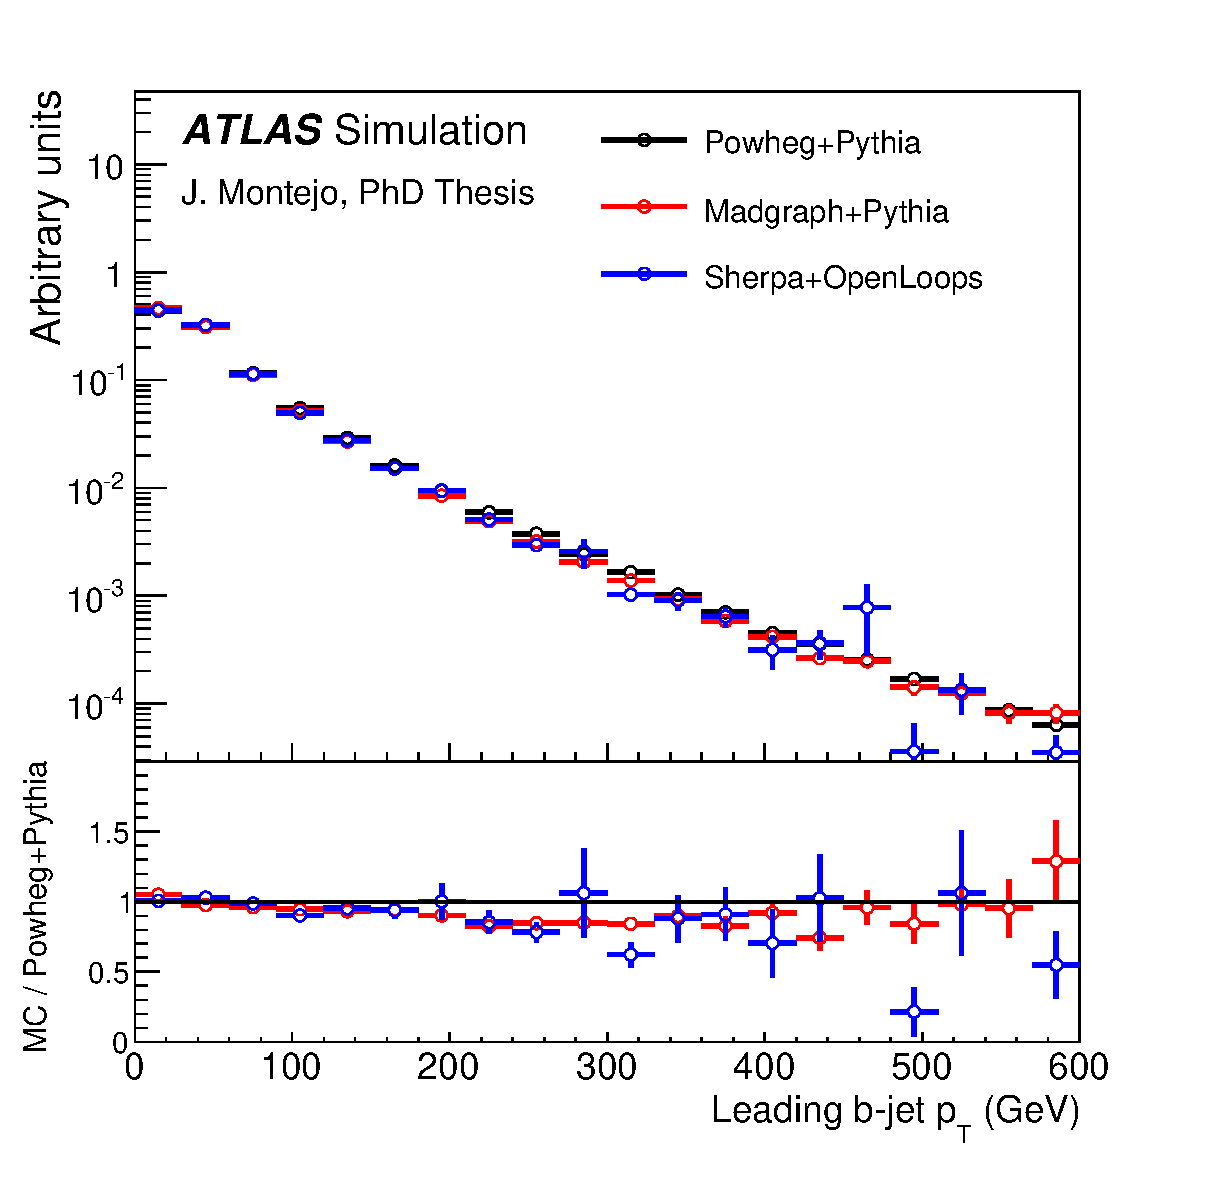
\includegraphics[width=0.46\textwidth]{Modeling/Figures/default_tt1bq_q1_pt_norm} &
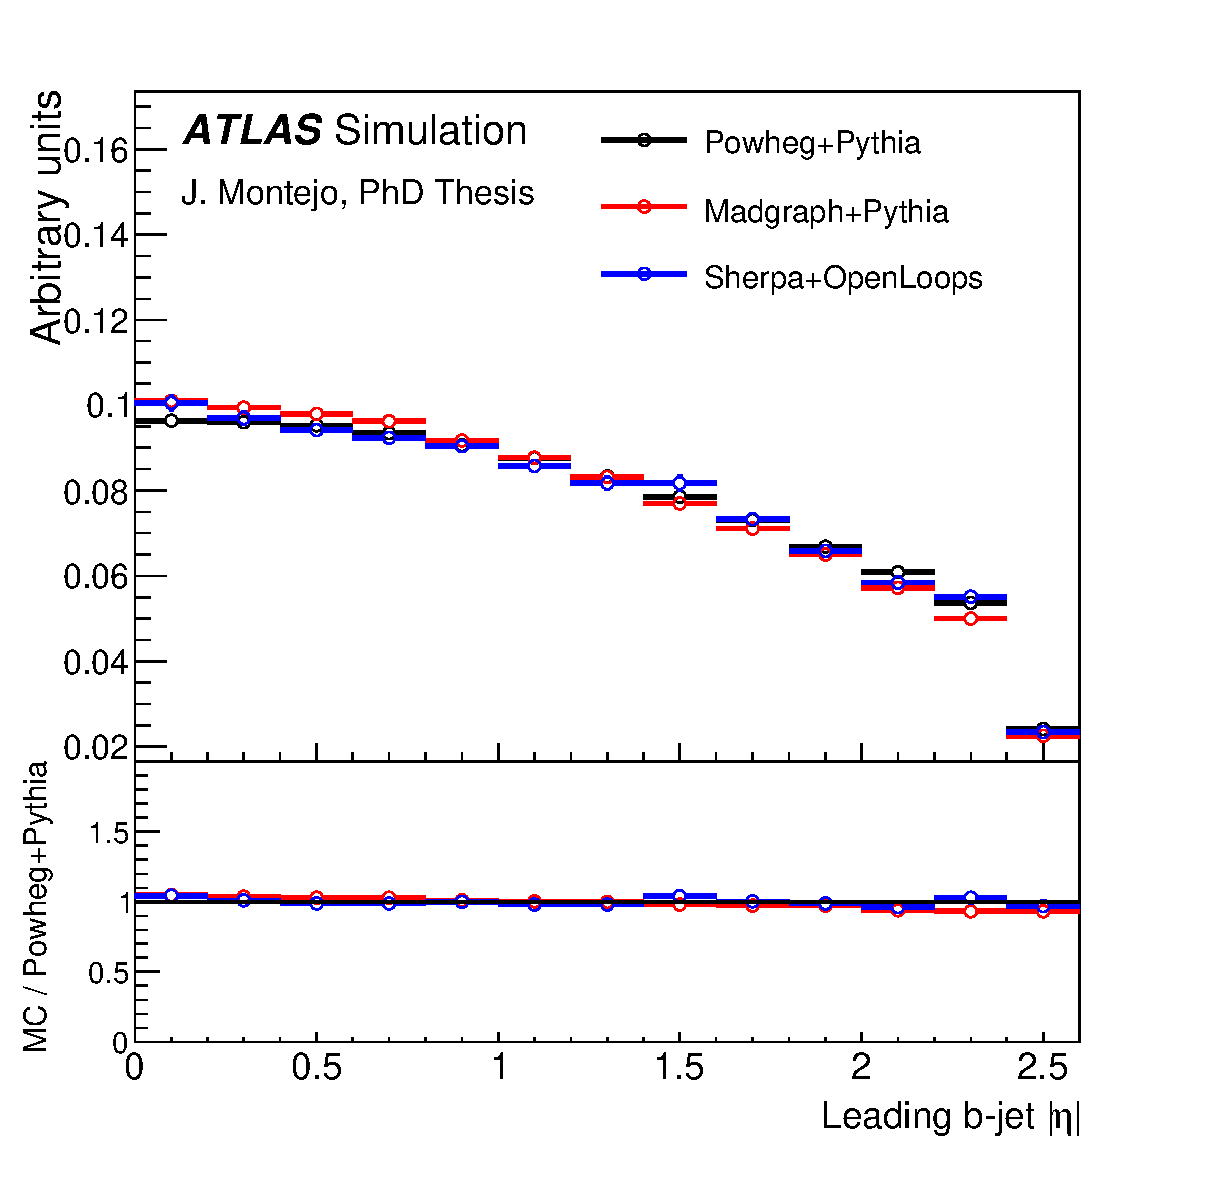
\includegraphics[width=0.46\textwidth]{Modeling/Figures/default_tt1bq_q1_eta_norm} \\
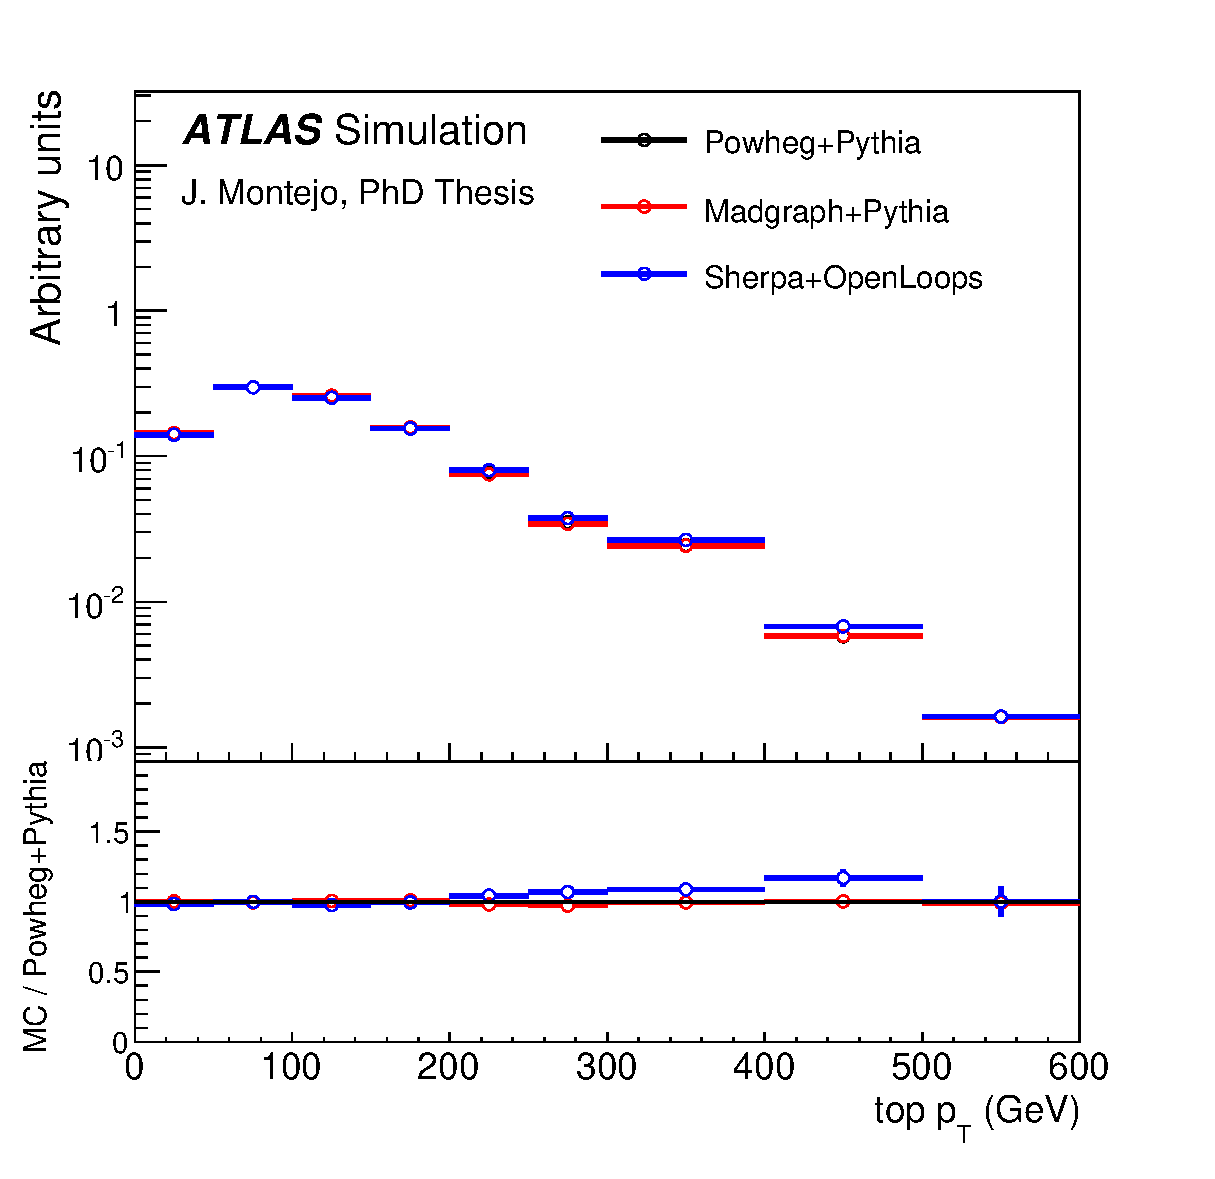
\includegraphics[width=0.46\textwidth]{Modeling/Figures/default_tt1bq_top_pt_norm} &
\includegraphics[width=0.46\textwidth]{Modeling/Figures/default_tt1bq_ttbar_pt_norm} \\
\end{tabular}
\caption{Comparison of kinematic variables in the $t\bar{t}+b$ topology between \PP, \madgraph+\pythia\ and \ShOL.}
\label{fig:default_tt1b}
\end{center}
\end{figure}
\begin{figure}[p]
\begin{center}
\begin{tabular}{cc}
\includegraphics[width=0.48\textwidth]{Modeling/Figures/default_tt1gbbq_q1_pt_norm} &
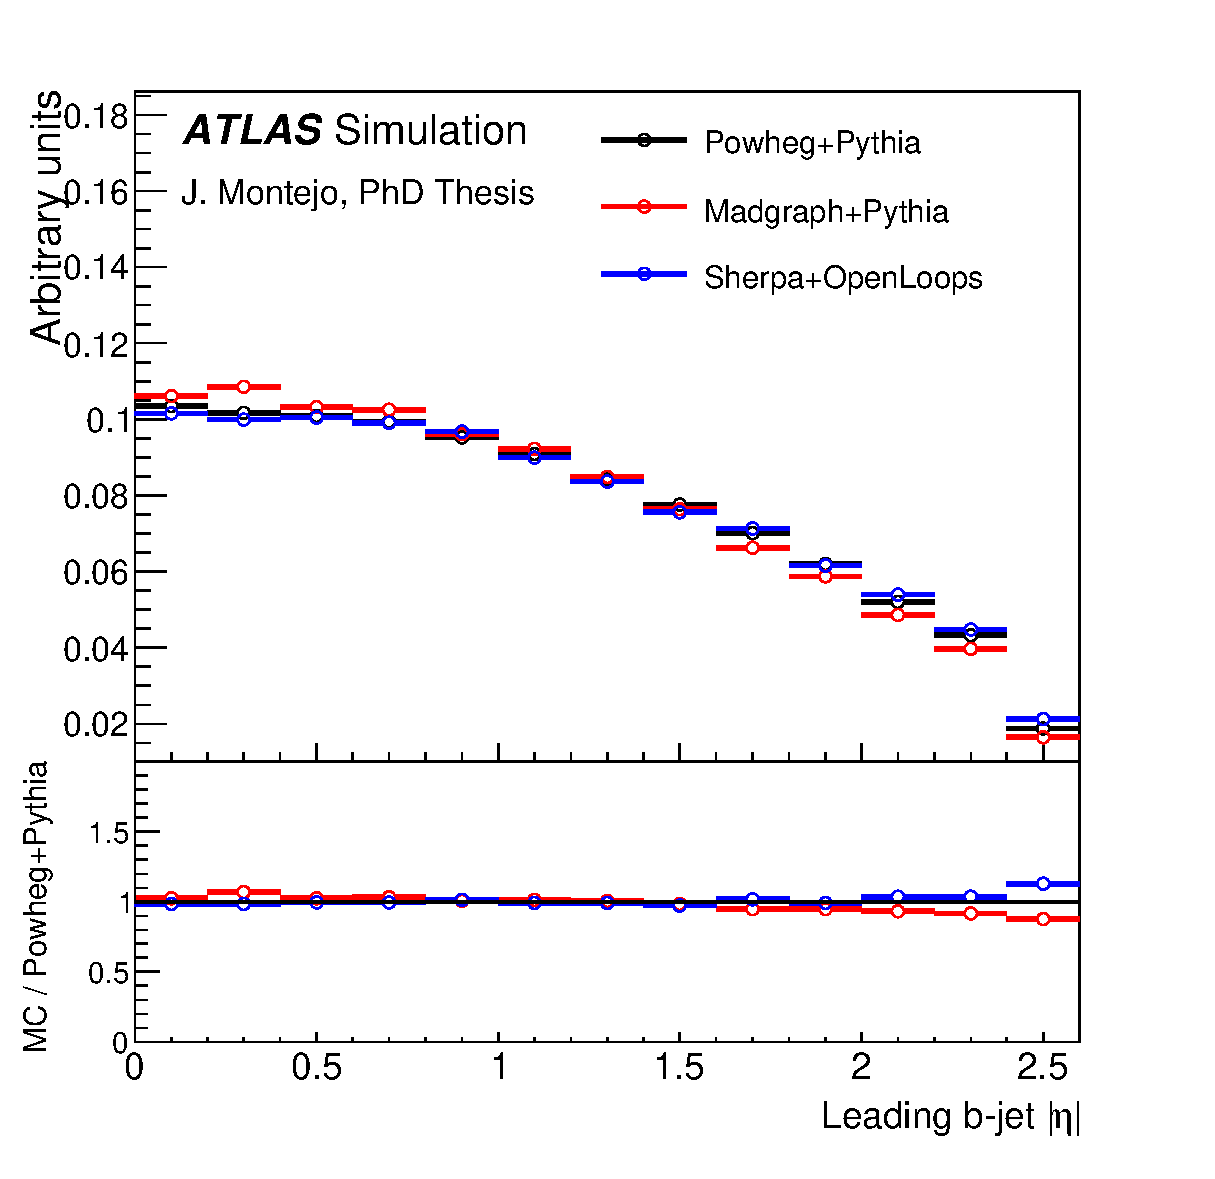
\includegraphics[width=0.48\textwidth]{Modeling/Figures/default_tt1gbbq_q1_eta_norm} \\
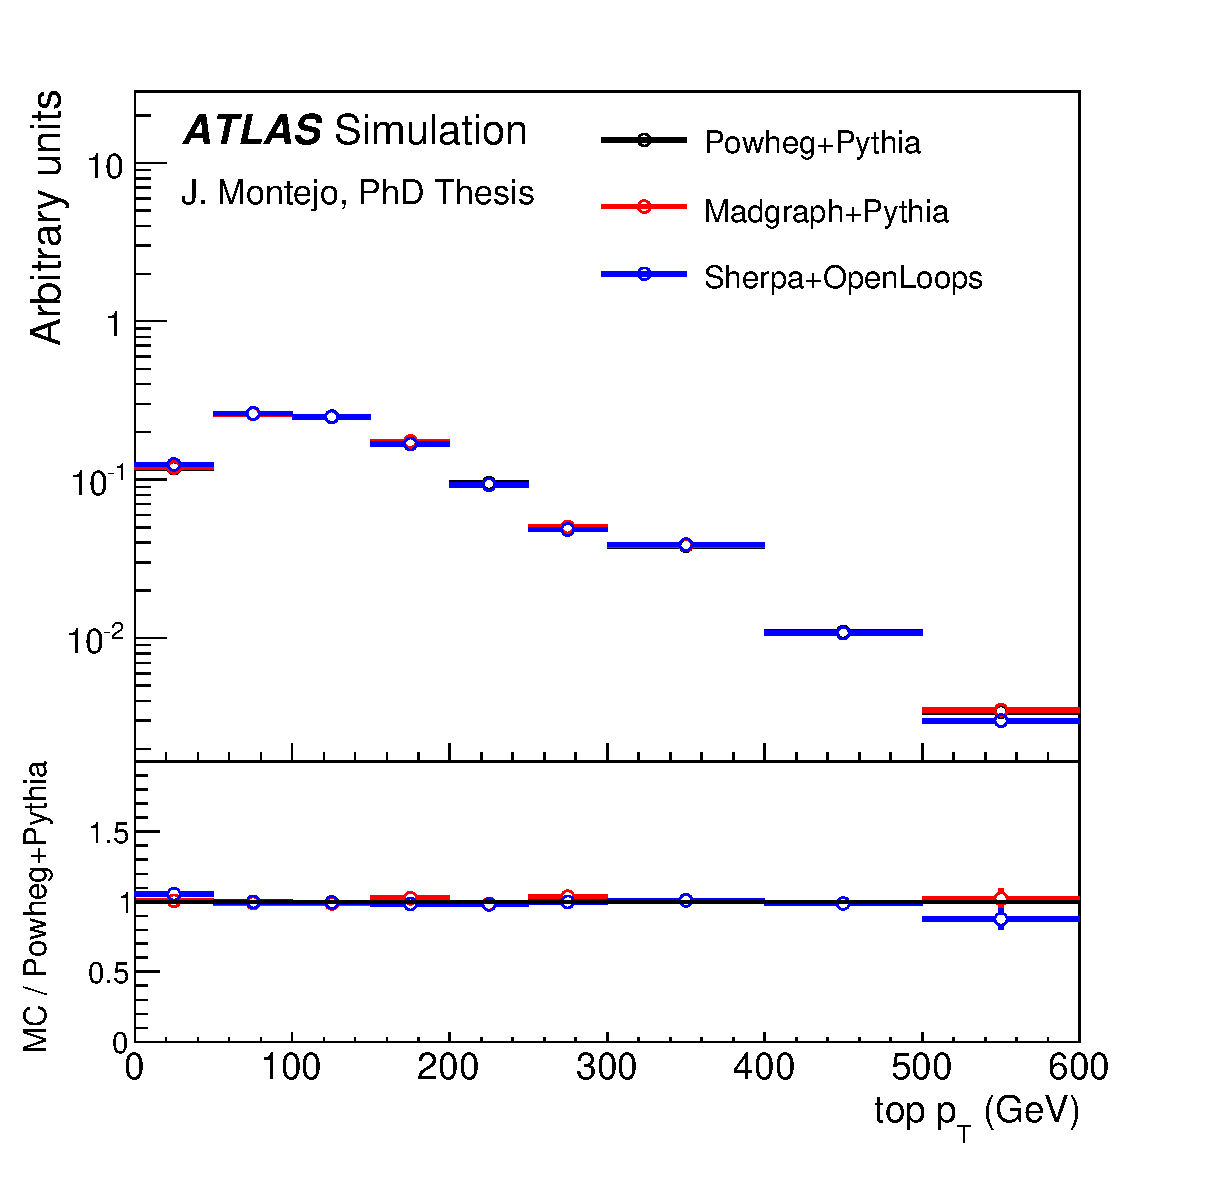
\includegraphics[width=0.48\textwidth]{Modeling/Figures/default_tt1gbbq_top_pt_norm} &
\includegraphics[width=0.48\textwidth]{Modeling/Figures/default_tt1gbbq_ttbar_pt_norm} \\
\end{tabular}
\caption{Comparison of kinematic variables in the $t\bar{t}+B$ topology between \PP, \madgraph+\pythia\ and \ShOL.}
\label{fig:default_tt1gbb}
\end{center}
\end{figure}
\begin{figure}[p]
\begin{center}
\begin{tabular}{cc}
\includegraphics[width=0.48\textwidth]{Modeling/Figures/default_tt2bq_q1_pt_norm} &
\includegraphics[width=0.48\textwidth]{Modeling/Figures/default_tt2bq_q1_eta_norm} \\
\includegraphics[width=0.48\textwidth]{Modeling/Figures/default_tt2bq_top_pt_norm} &
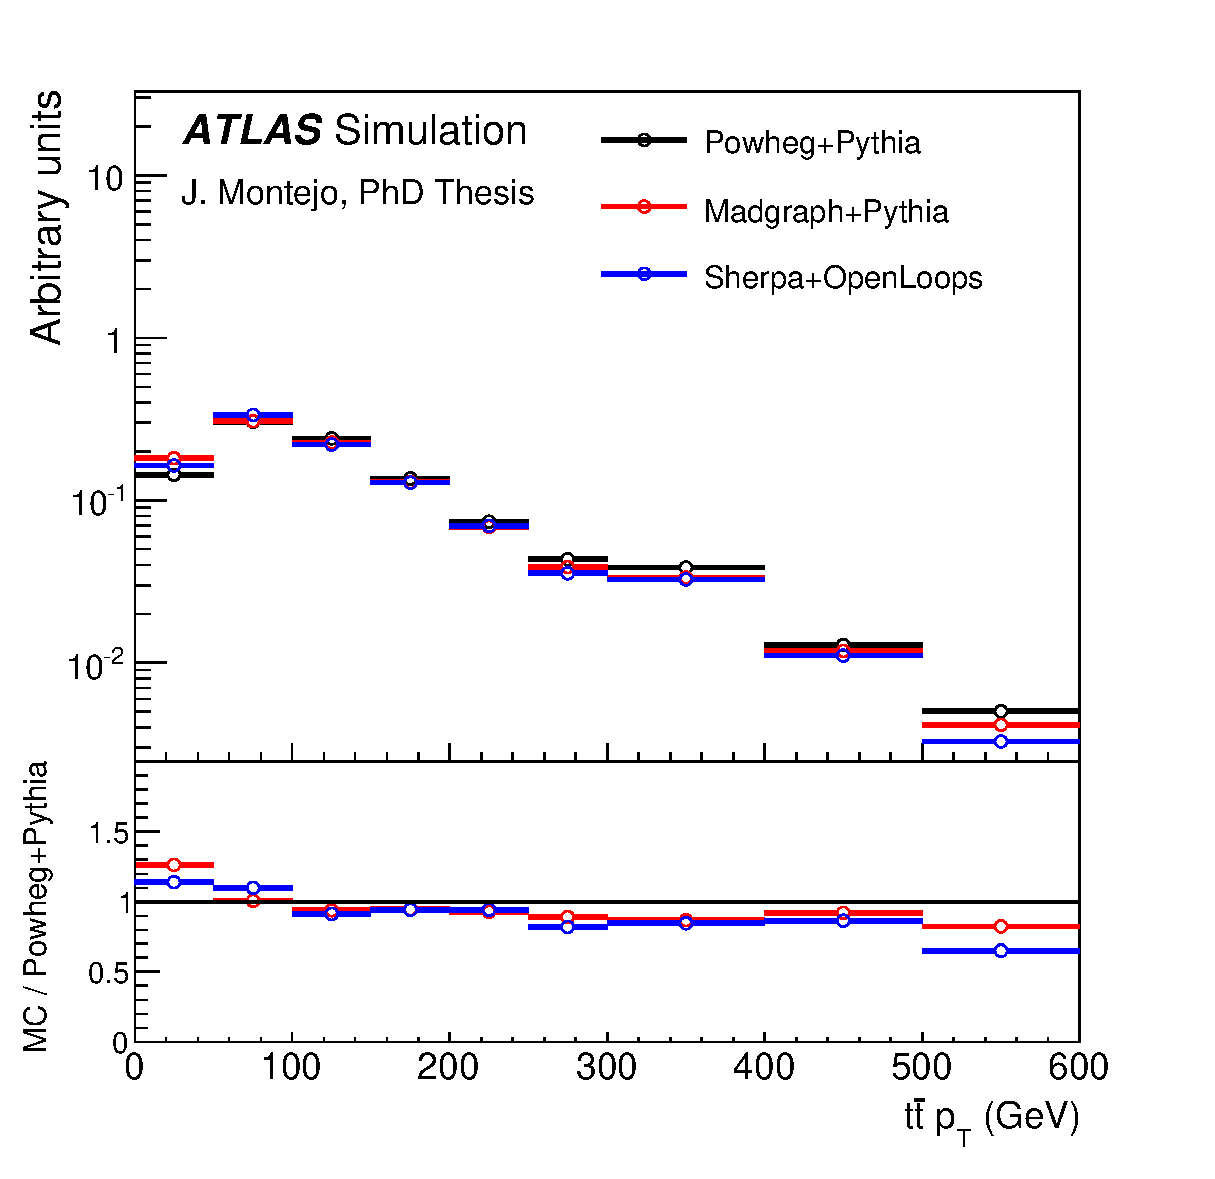
\includegraphics[width=0.48\textwidth]{Modeling/Figures/default_tt2bq_ttbar_pt_norm} \\
\end{tabular}
\caption{Comparison of kinematic variables in the $t\bar{t}+bb$ topology between \PP, \madgraph+\pythia\ and \ShOL.}
\label{fig:default_tt2b}
\end{center}
\end{figure}
\begin{figure}[p]
\begin{center}
\begin{tabular}{cc}
\includegraphics[width=0.48\textwidth]{Modeling/Figures/default_tt2bq_qq_m_norm} &
\includegraphics[width=0.48\textwidth]{Modeling/Figures/default_tt2bq_qq_pt_norm} \\
\includegraphics[width=0.48\textwidth]{Modeling/Figures/default_tt2bq_qq_dr_norm} &
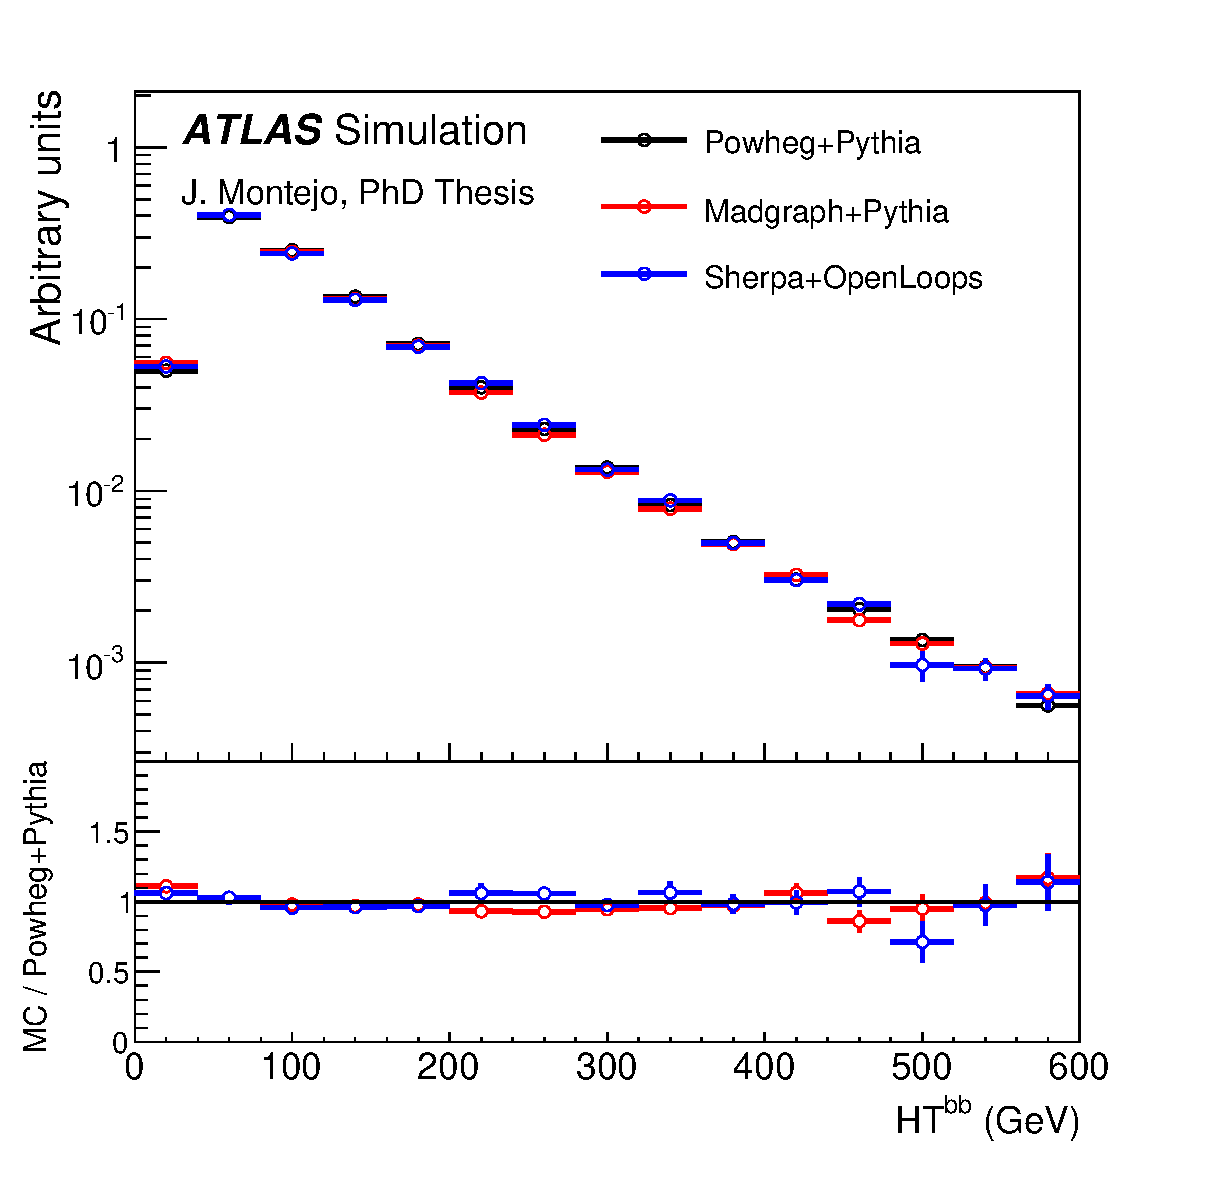
\includegraphics[width=0.48\textwidth]{Modeling/Figures/default_tt2bq_qq_ht_norm} \\
\end{tabular}
\caption{Comparison of kinematic variables of the \bbbar\ system in the $t\bar{t}+bb$ topology between \PP, \madgraph+\pythia\ and \ShOL.}
\label{fig:default_tt2b_bb}
\end{center}
\end{figure}
%%%%%%%%%%%%%%% MG/PP ME vs PS
\begin{figure}[tp]
\centering
\begin{tabular}{cc}
  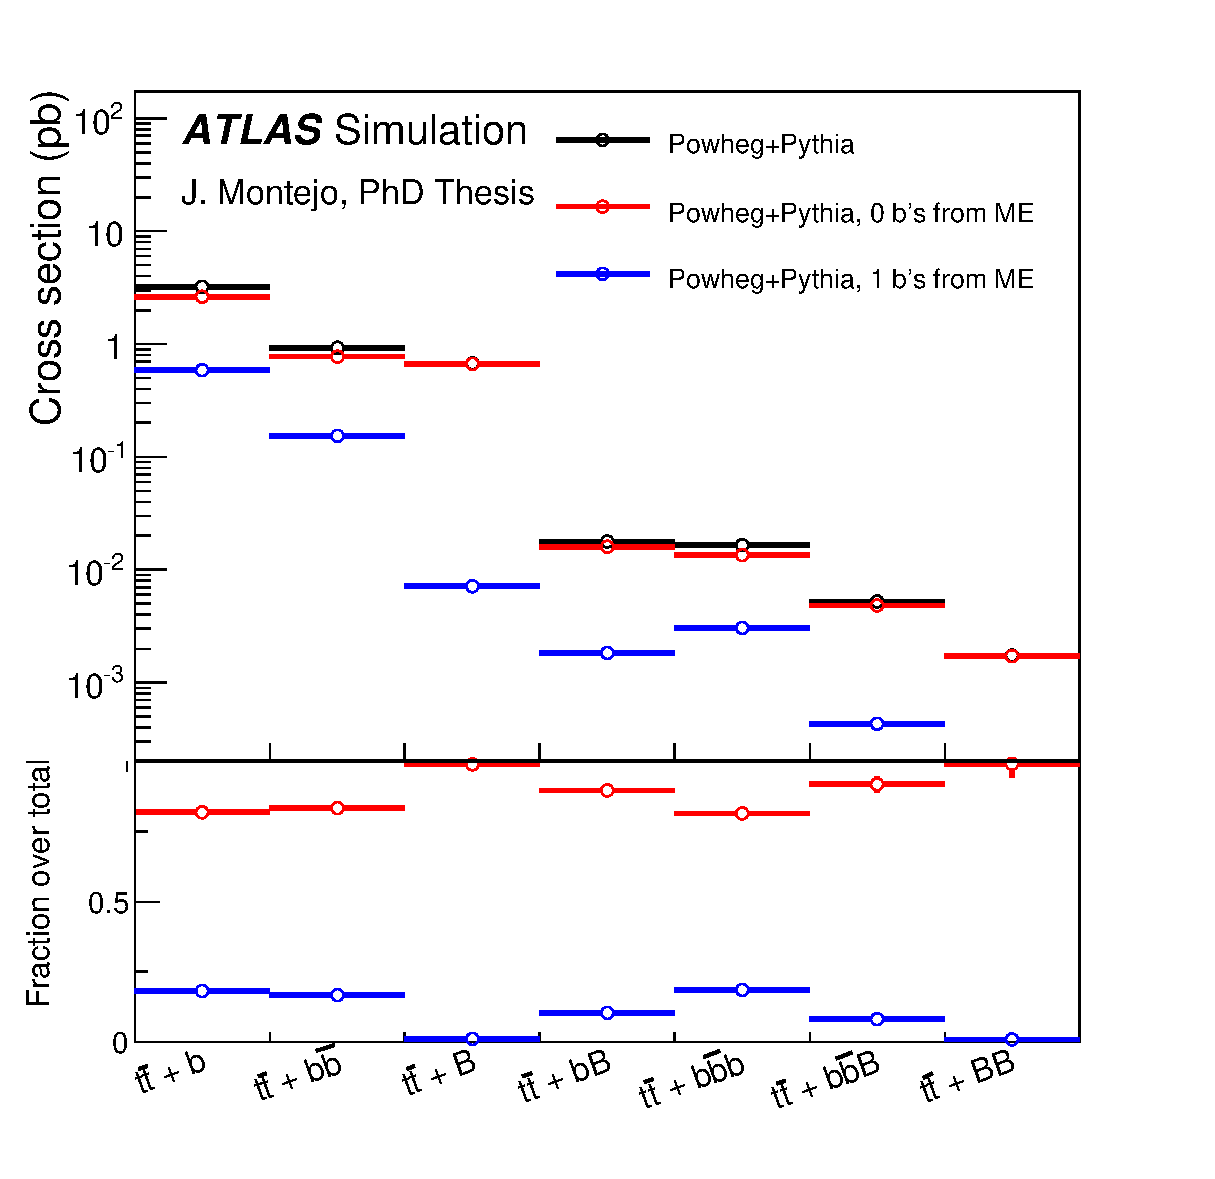
\includegraphics[width=0.47\textwidth]{Modeling/Figures/mepspp_realHFbb_extHFtype.eps} &
  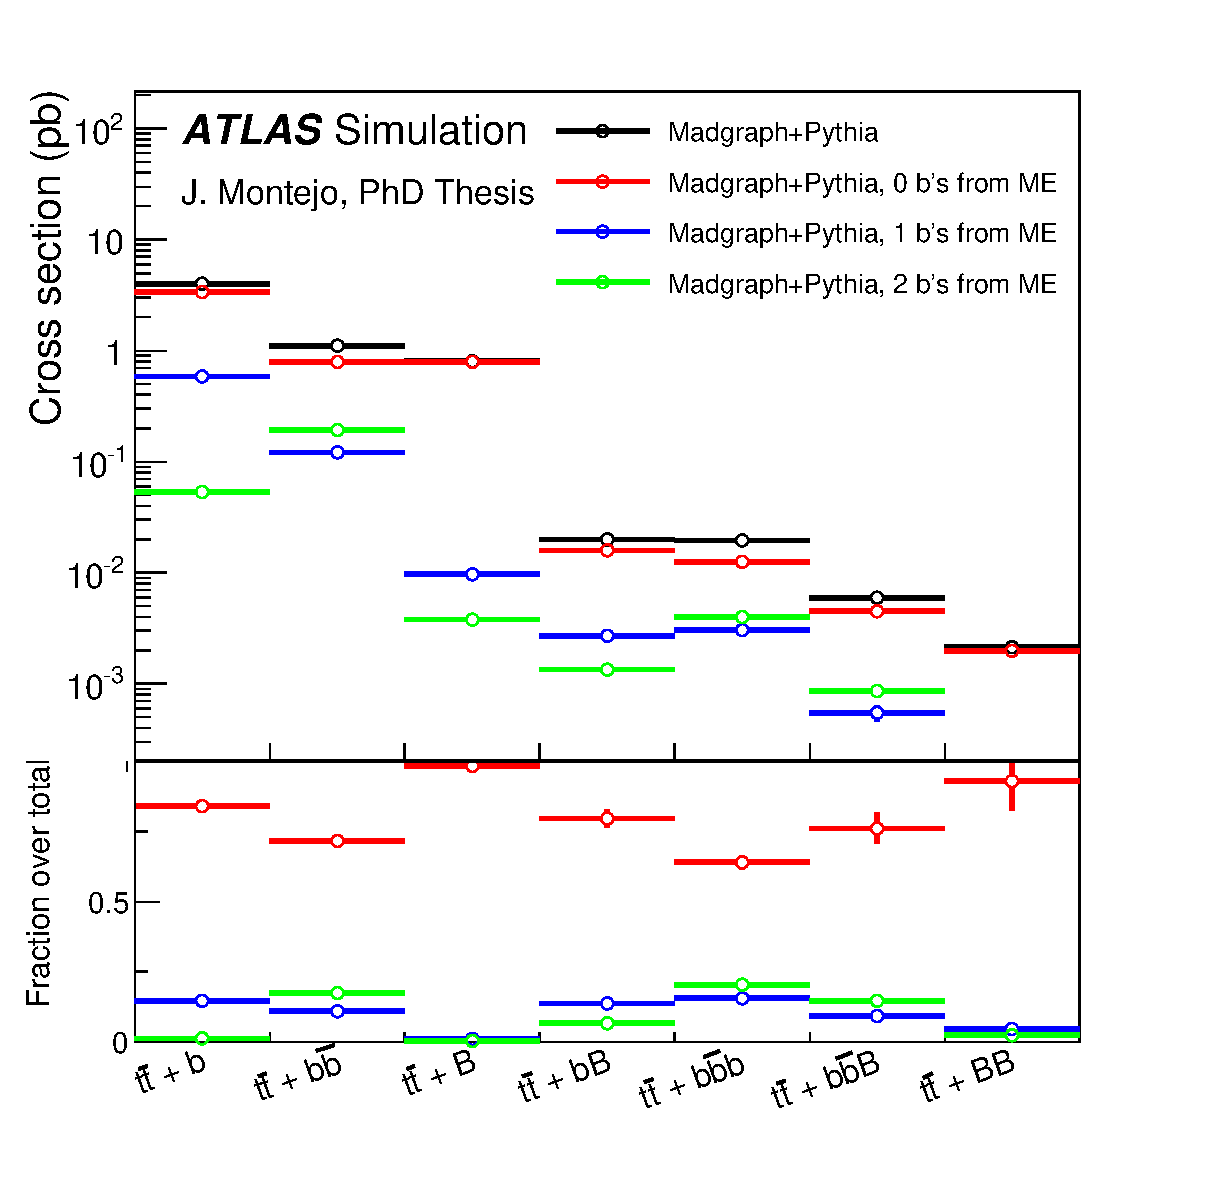
\includegraphics[width=0.47\textwidth]{Modeling/Figures/meps_realHFbb_extHFtype.eps} \\
  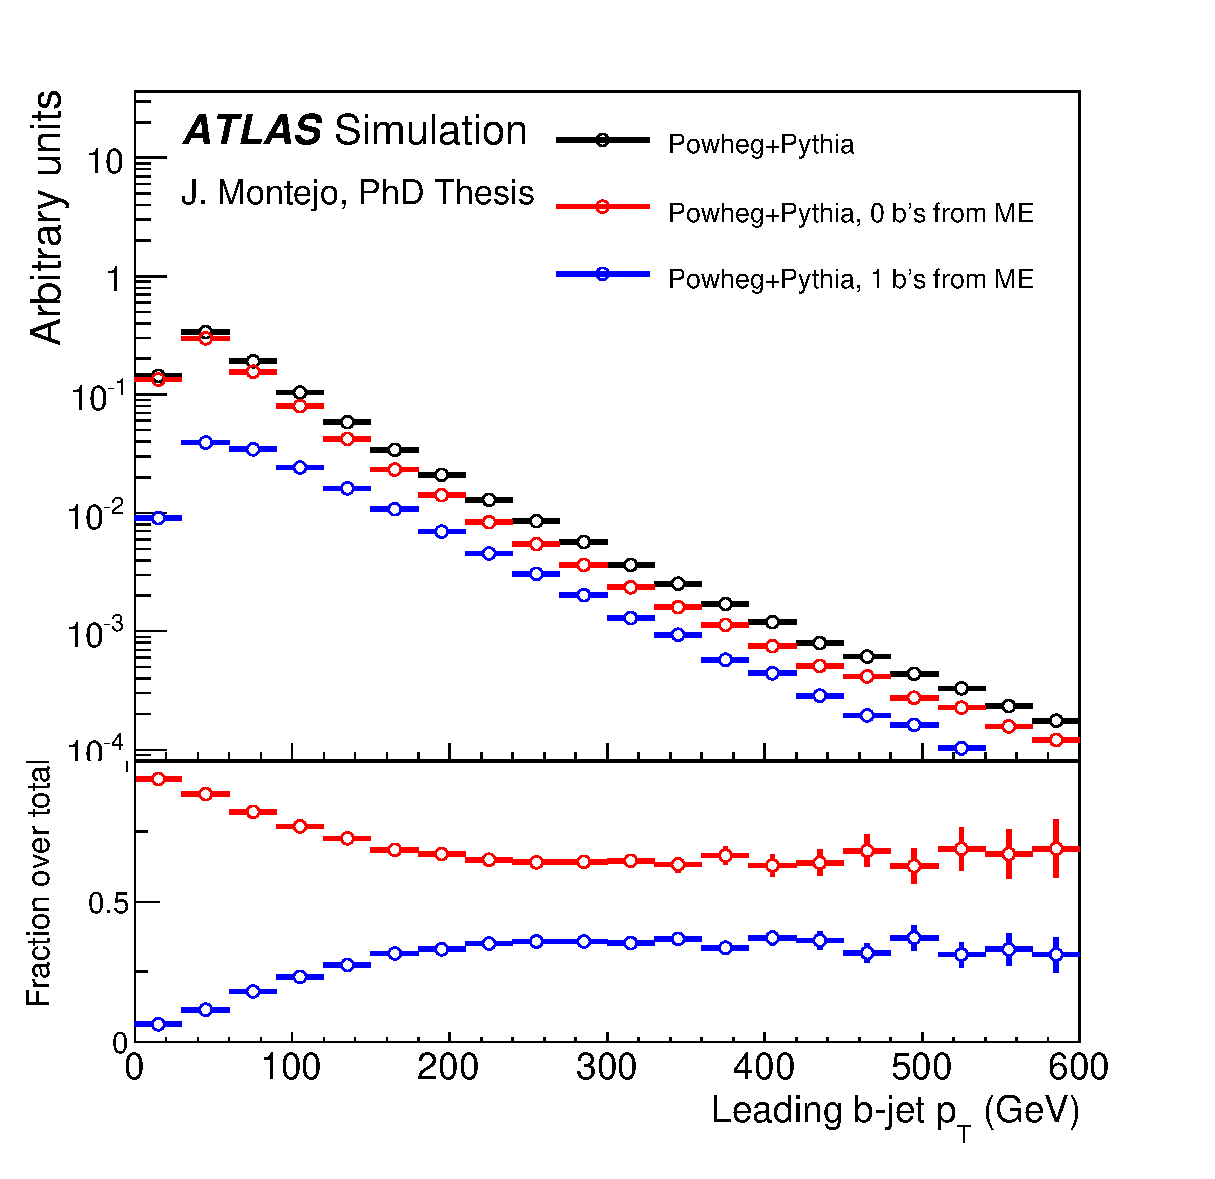
\includegraphics[width=0.47\textwidth]{Modeling/Figures/mepspp_tt2bq_q1_pt.eps} & 
  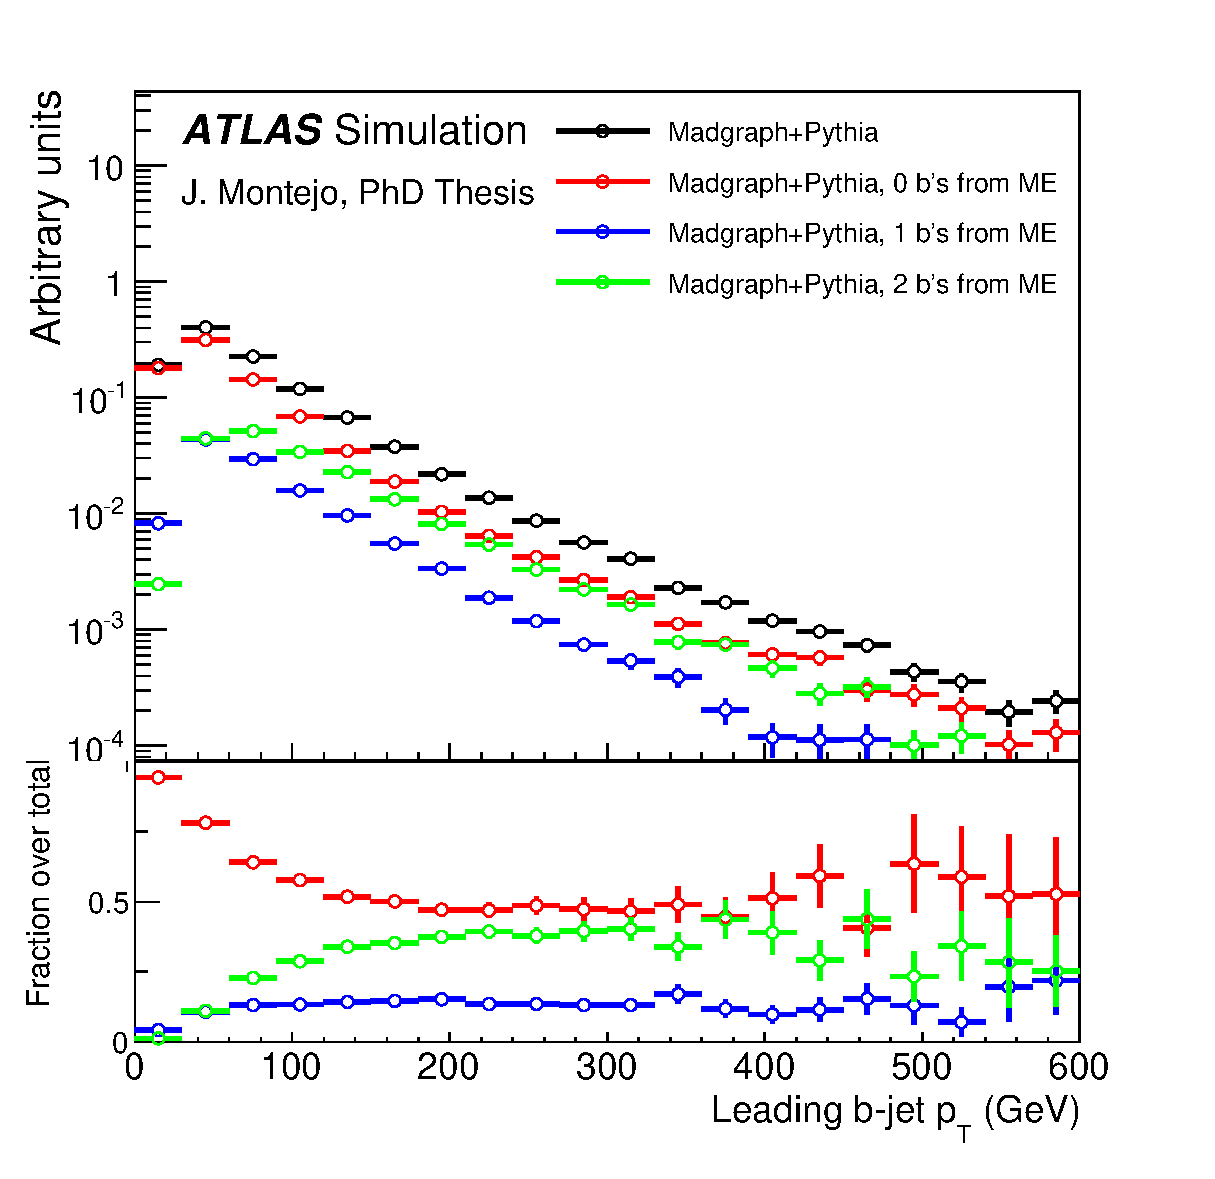
\includegraphics[width=0.47\textwidth]{Modeling/Figures/meps_tt2bq_q1_pt.eps} \\
  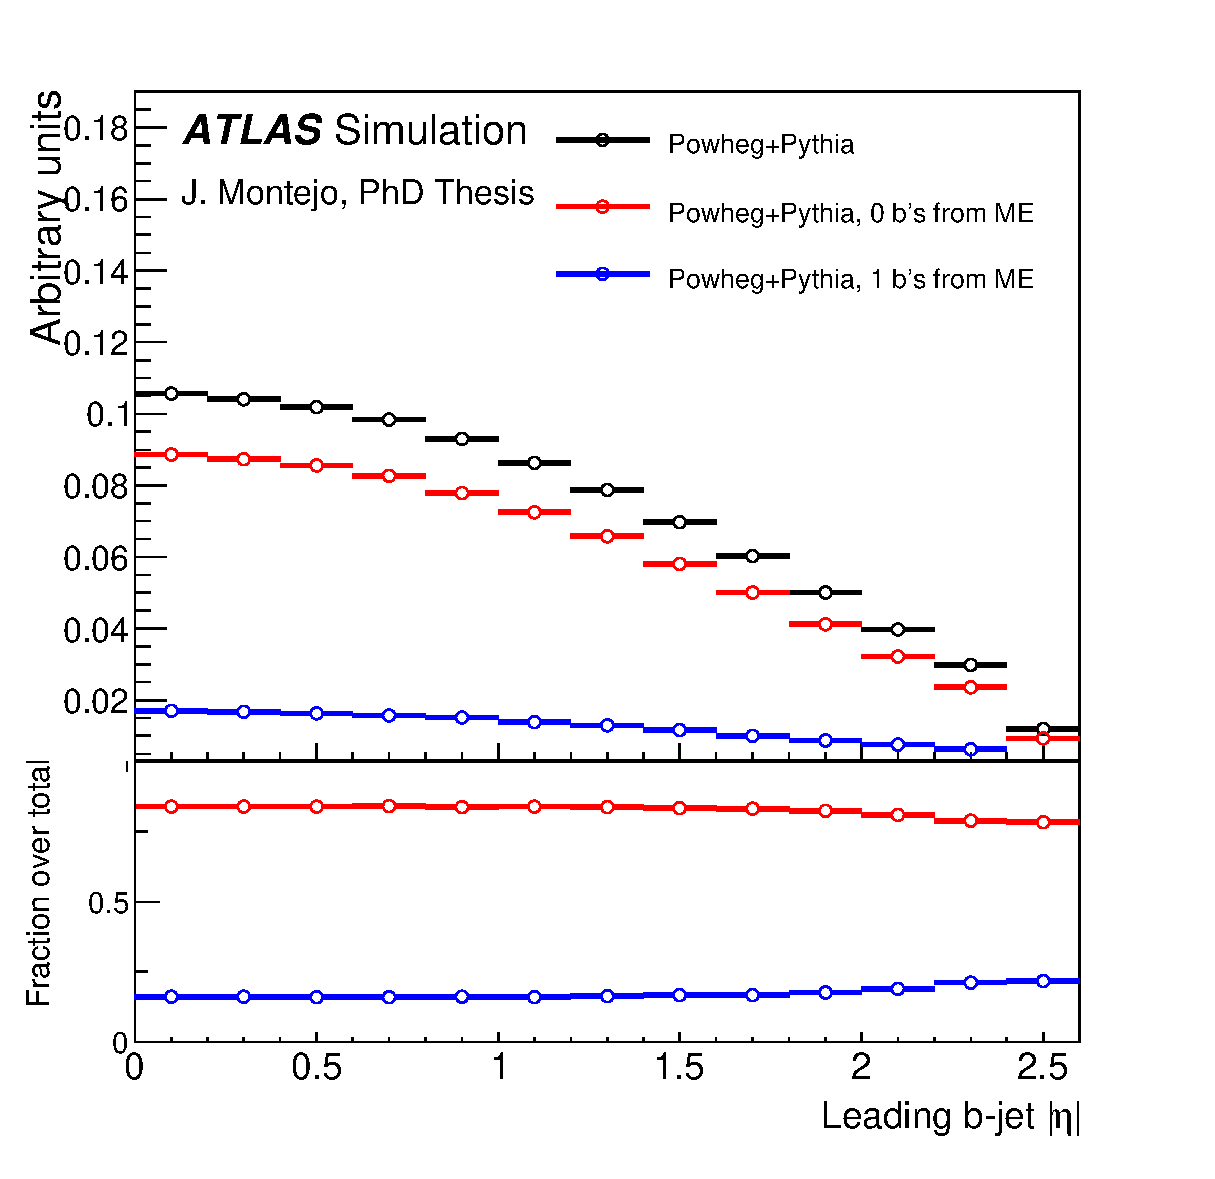
\includegraphics[width=0.47\textwidth]{Modeling/Figures/mepspp_tt2bq_q1_eta.eps} & 
  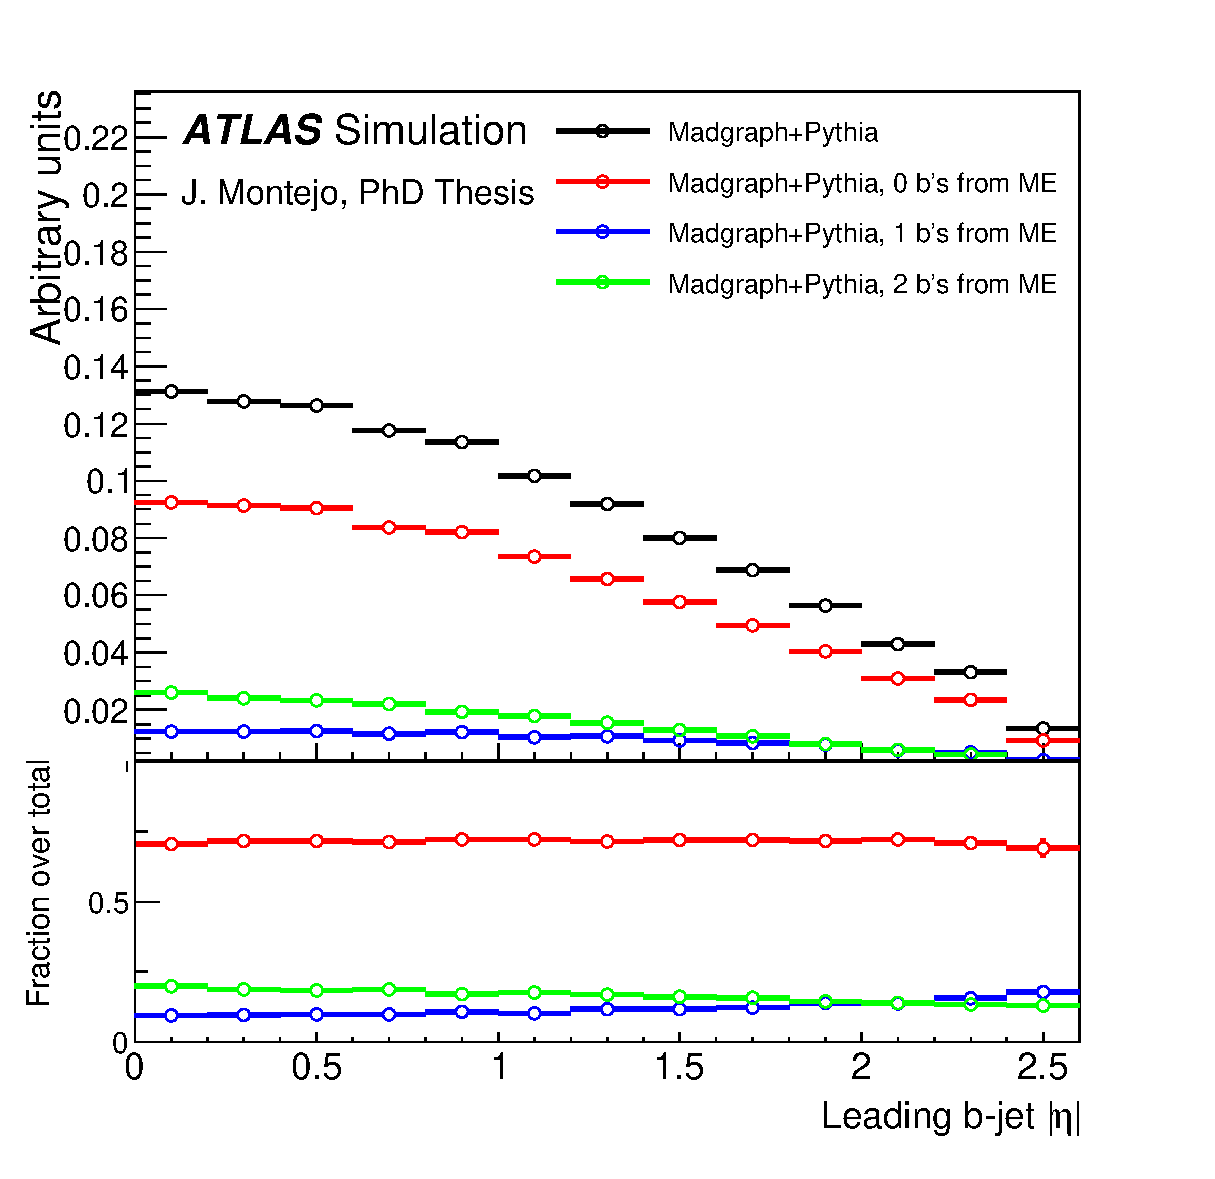
\includegraphics[width=0.47\textwidth]{Modeling/Figures/meps_tt2bq_q1_eta.eps} \\
\end{tabular}
  \caption{Comparison of kinematic variables between \PP\ and \madgraph+\pythia (left) and fractions of the \madgraph\ prediction split according to the number of $b$-quarks in the ME (right). 
  The variables displayed are: \ttbb\ subcategories (top), leading $b$-jet \pt\ in \ttbb\ (middle) and leading $b$-jet \eta\ in \ttbb.}
  \label{fig:mgpp_splitME_1}
\end{figure}
\begin{figure}[tp]
\centering
\begin{tabular}{cc}
  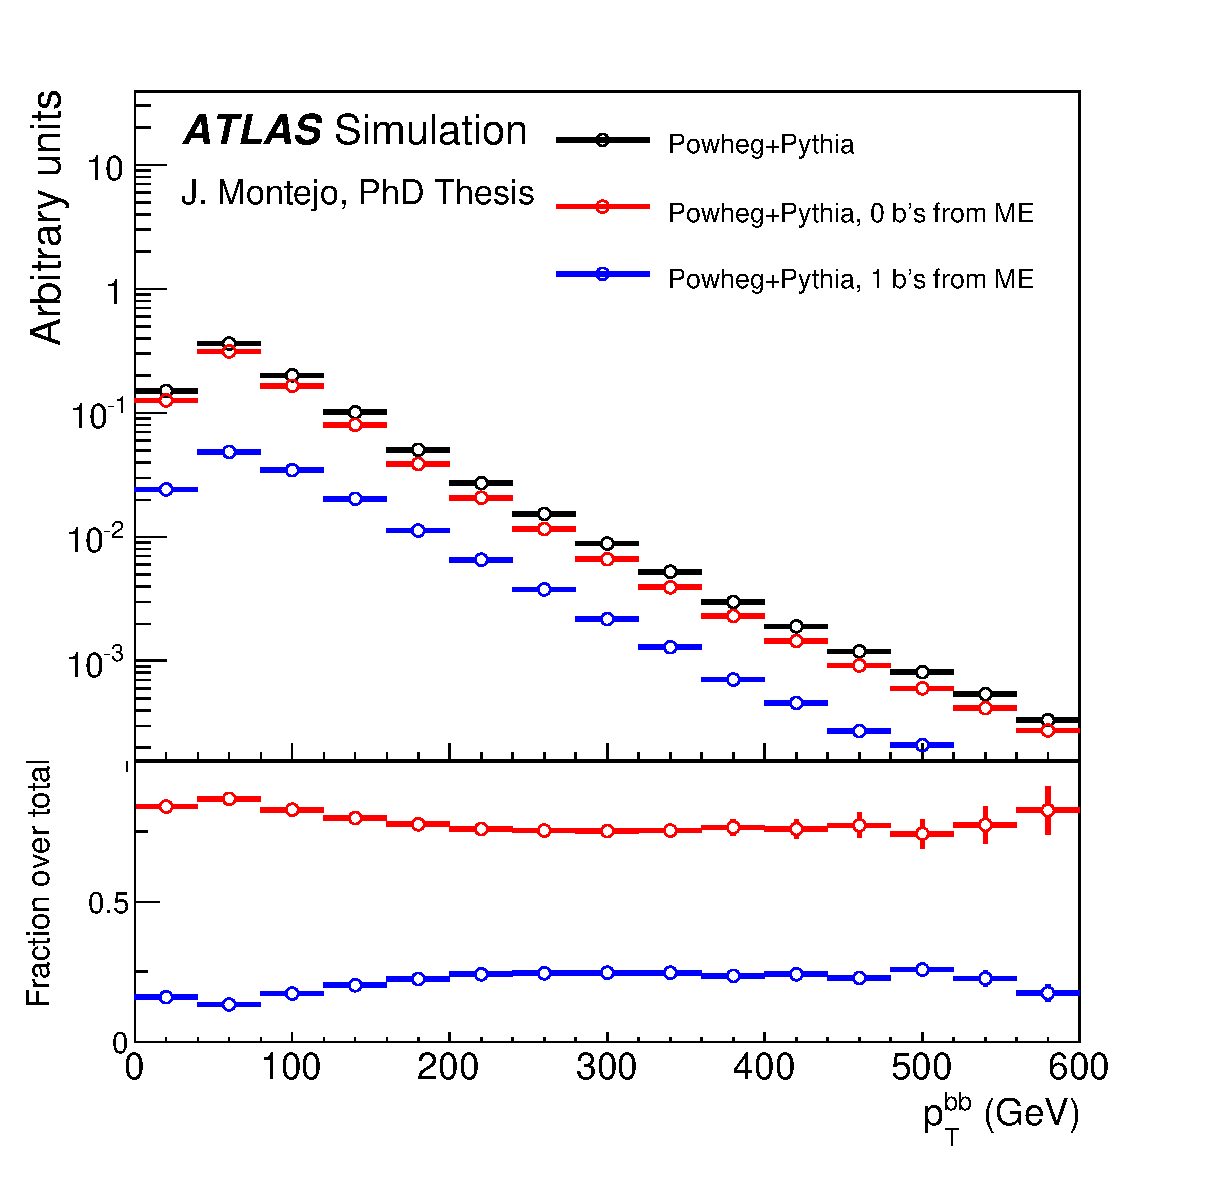
\includegraphics[width=0.47\textwidth]{Modeling/Figures/mepspp_tt2bq_qq_pt.eps} & 
  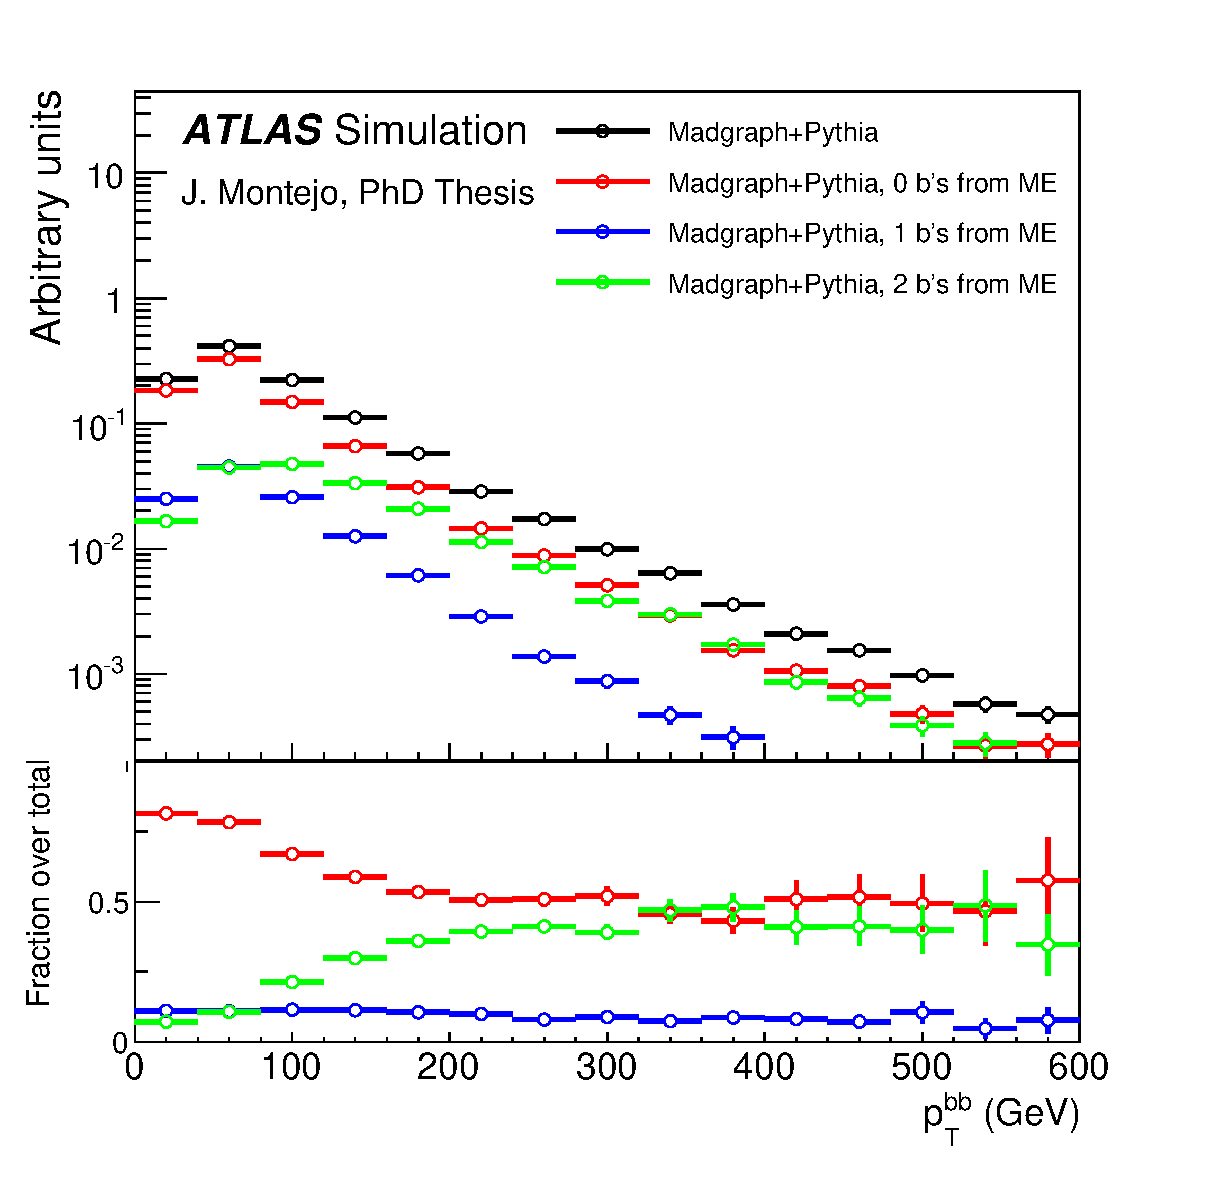
\includegraphics[width=0.47\textwidth]{Modeling/Figures/meps_tt2bq_qq_pt.eps} \\
  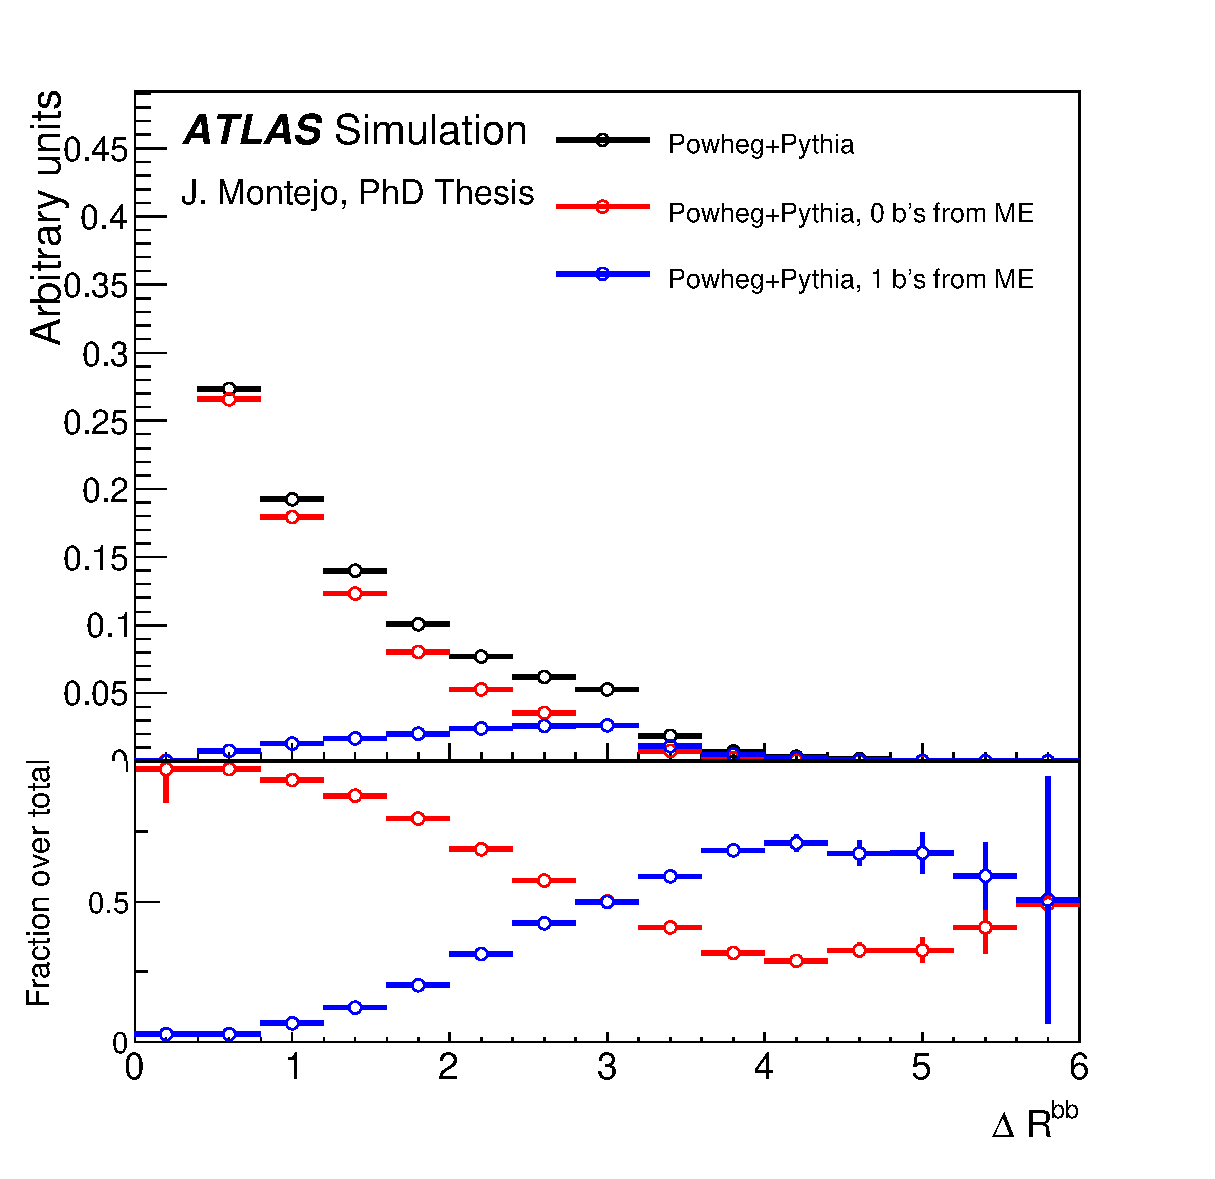
\includegraphics[width=0.47\textwidth]{Modeling/Figures/mepspp_tt2bq_qq_dr.eps} & 
  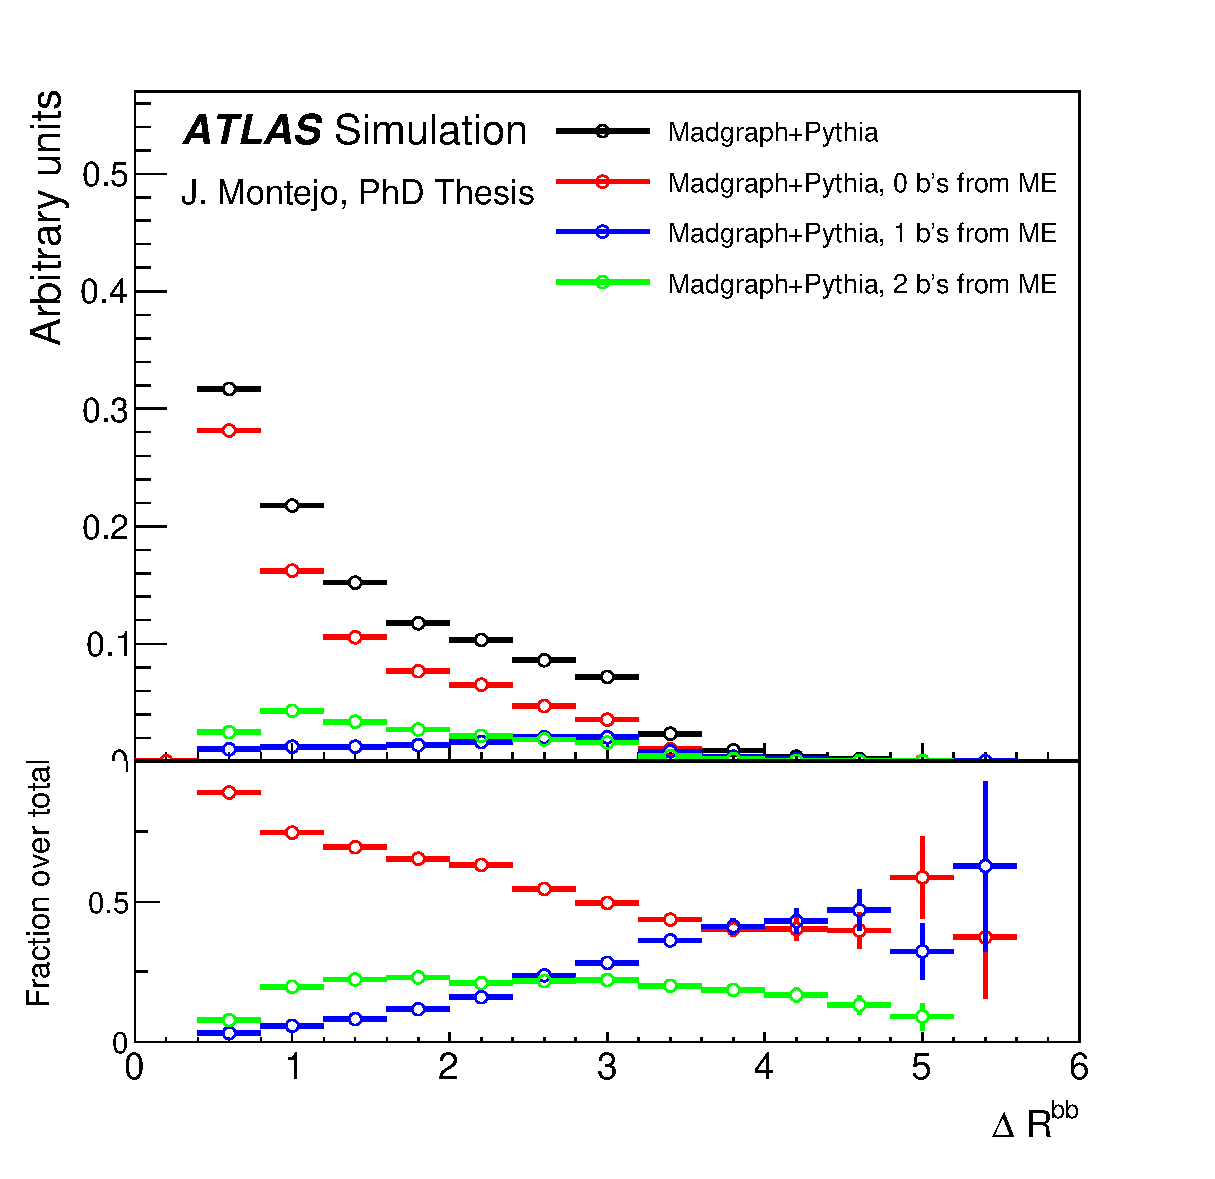
\includegraphics[width=0.47\textwidth]{Modeling/Figures/meps_tt2bq_qq_dr.eps} \\
  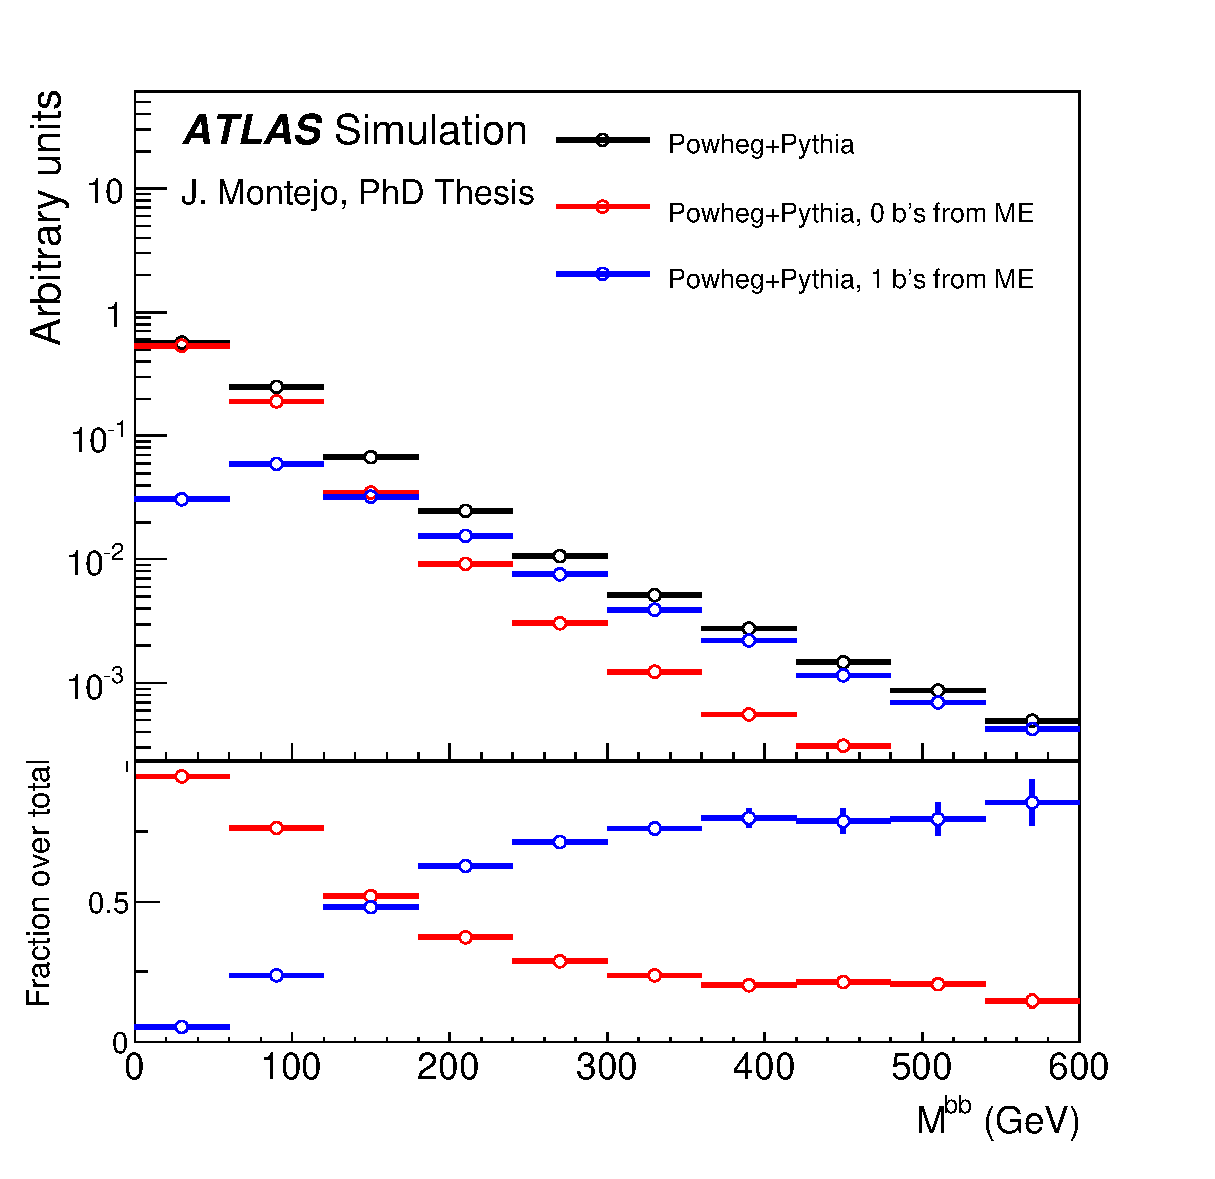
\includegraphics[width=0.47\textwidth]{Modeling/Figures/mepspp_tt2bq_qq_m.eps} & 
  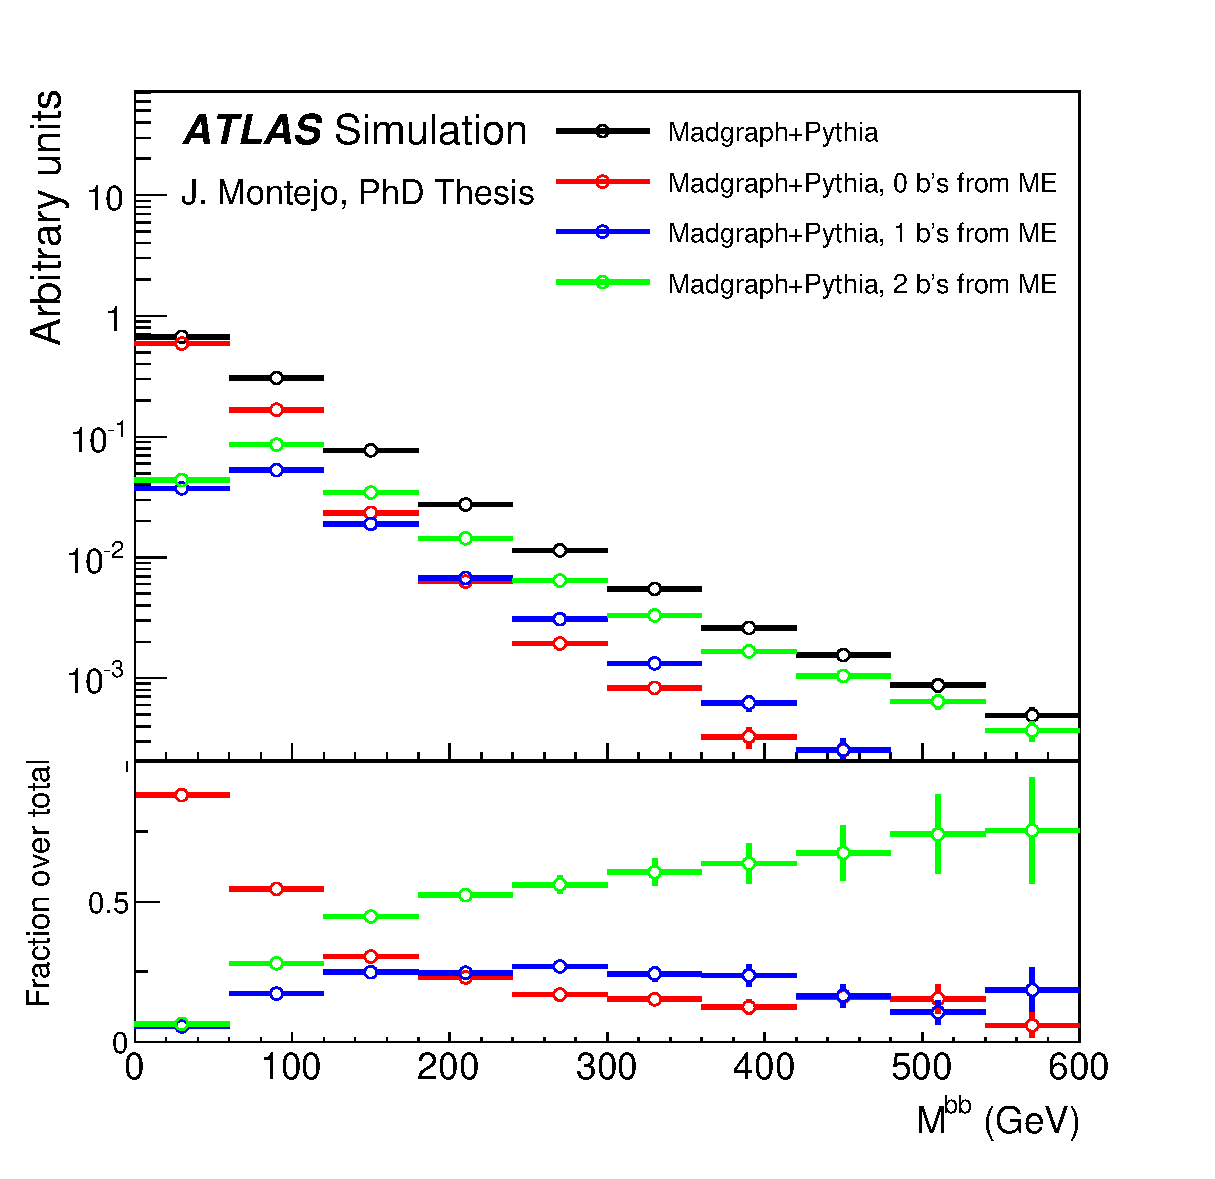
\includegraphics[width=0.47\textwidth]{Modeling/Figures/meps_tt2bq_qq_m.eps} \\
\end{tabular}
  \caption{Comparison of kinematic variables between \PP\ and \madgraph+\pythia (left) and fractions of the \madgraph\ prediction split according to the number of $b$-quarks in the ME (right). 
  The variables displayed are: \pt\ of the \bbbar\ system in \ttbb\ (top), \DR\ between the $b$-jets in \ttbb\ (middle) and mass of the \bbbar\ system in \ttbb.}
  \label{fig:mgpp_splitME_2}
\end{figure}
%%%%%%%%%%%%%%% ttbb reweighting
\begin{figure}[p]
\begin{center}
\begin{tabular}{cc}
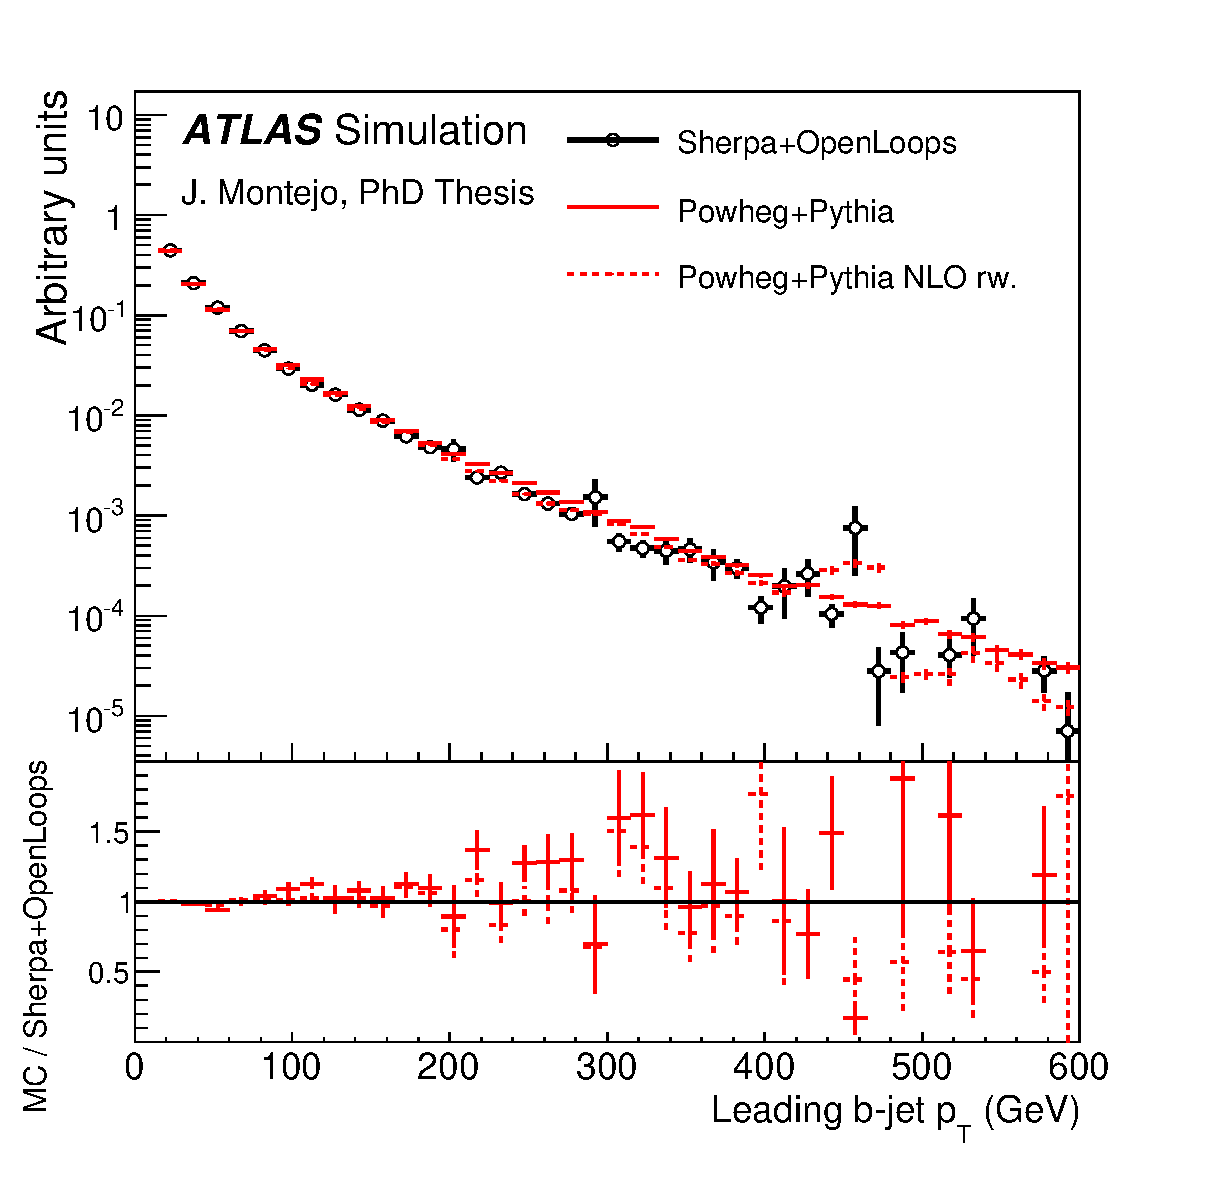
\includegraphics[width=0.48\textwidth]{Modeling/Figures/rw_tt1bq_q1_pt.eps} &
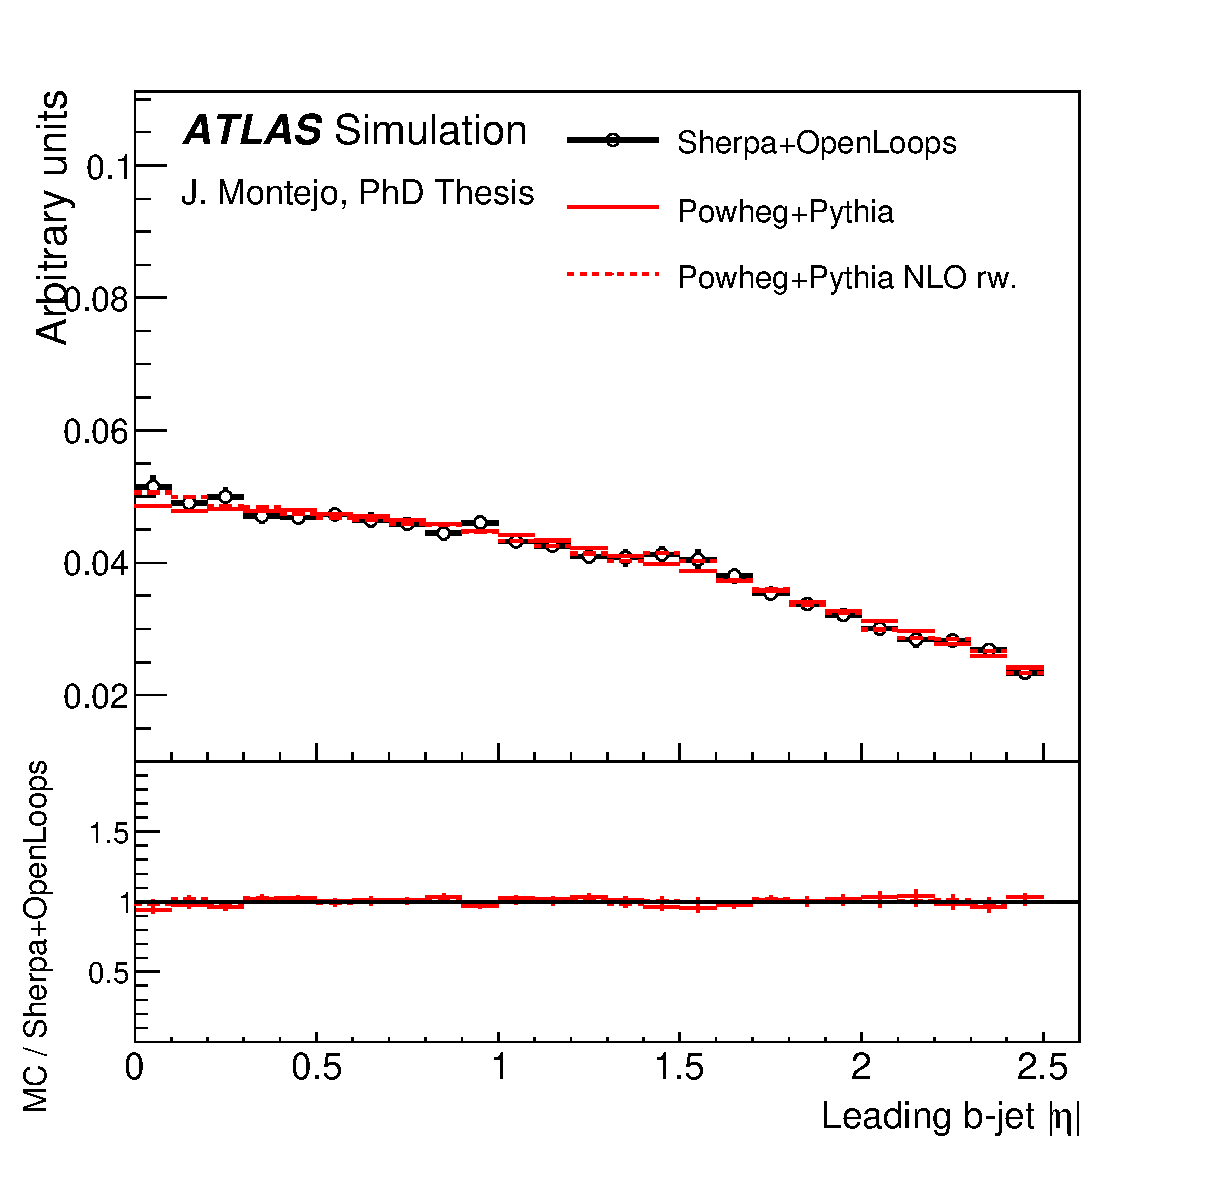
\includegraphics[width=0.48\textwidth]{Modeling/Figures/rw_tt1bq_q1_eta.eps} \\
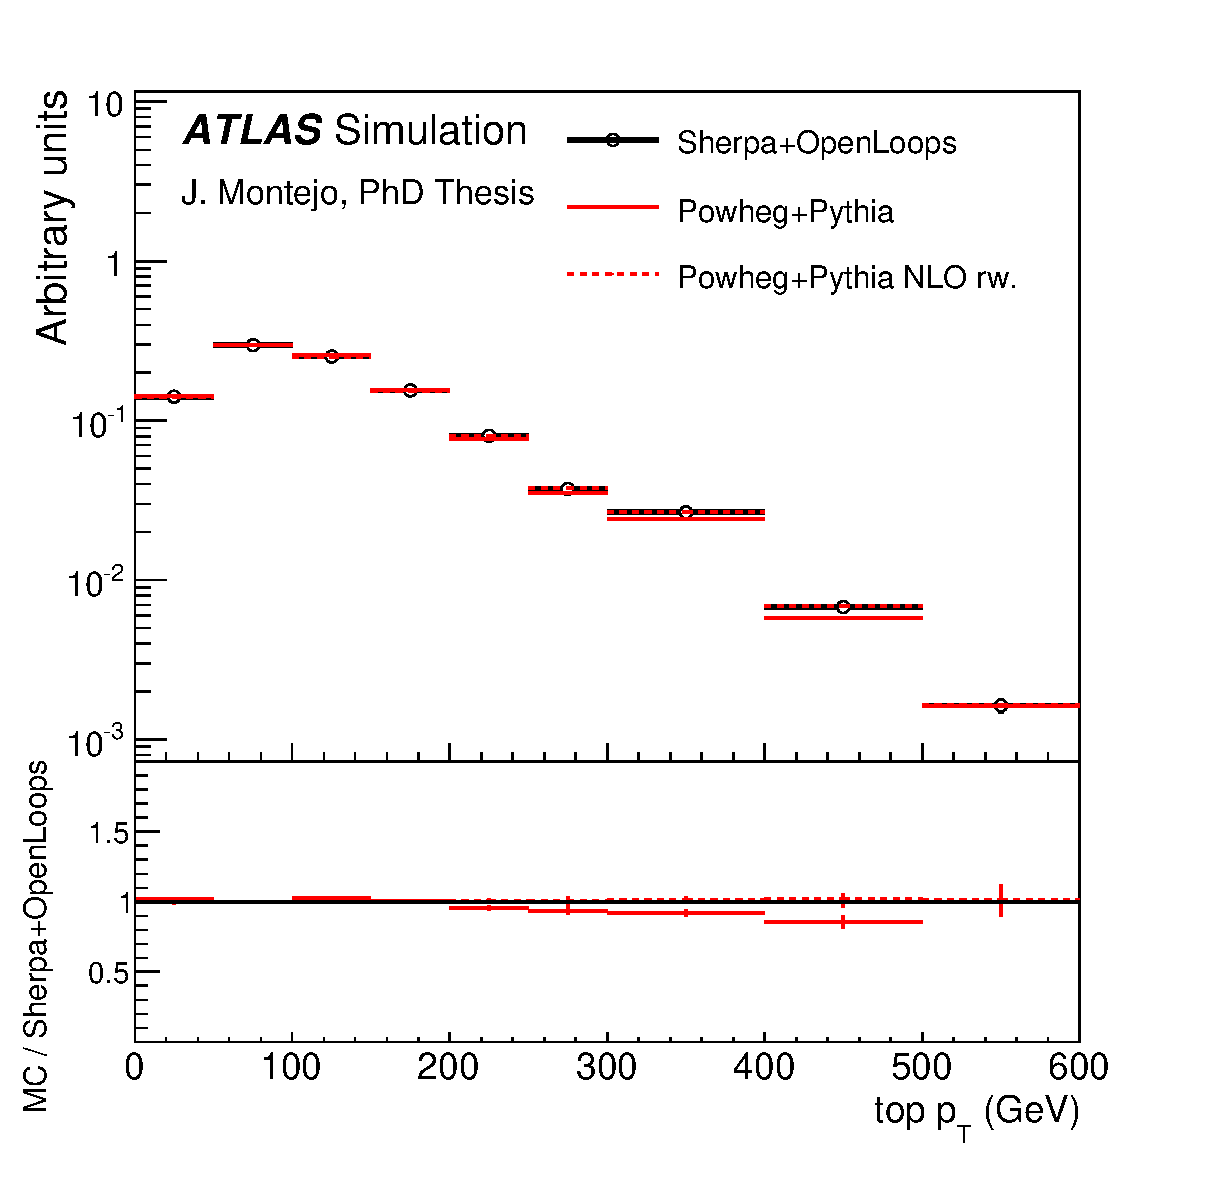
\includegraphics[width=0.48\textwidth]{Modeling/Figures/rw_tt1bq_top_pt.eps} &
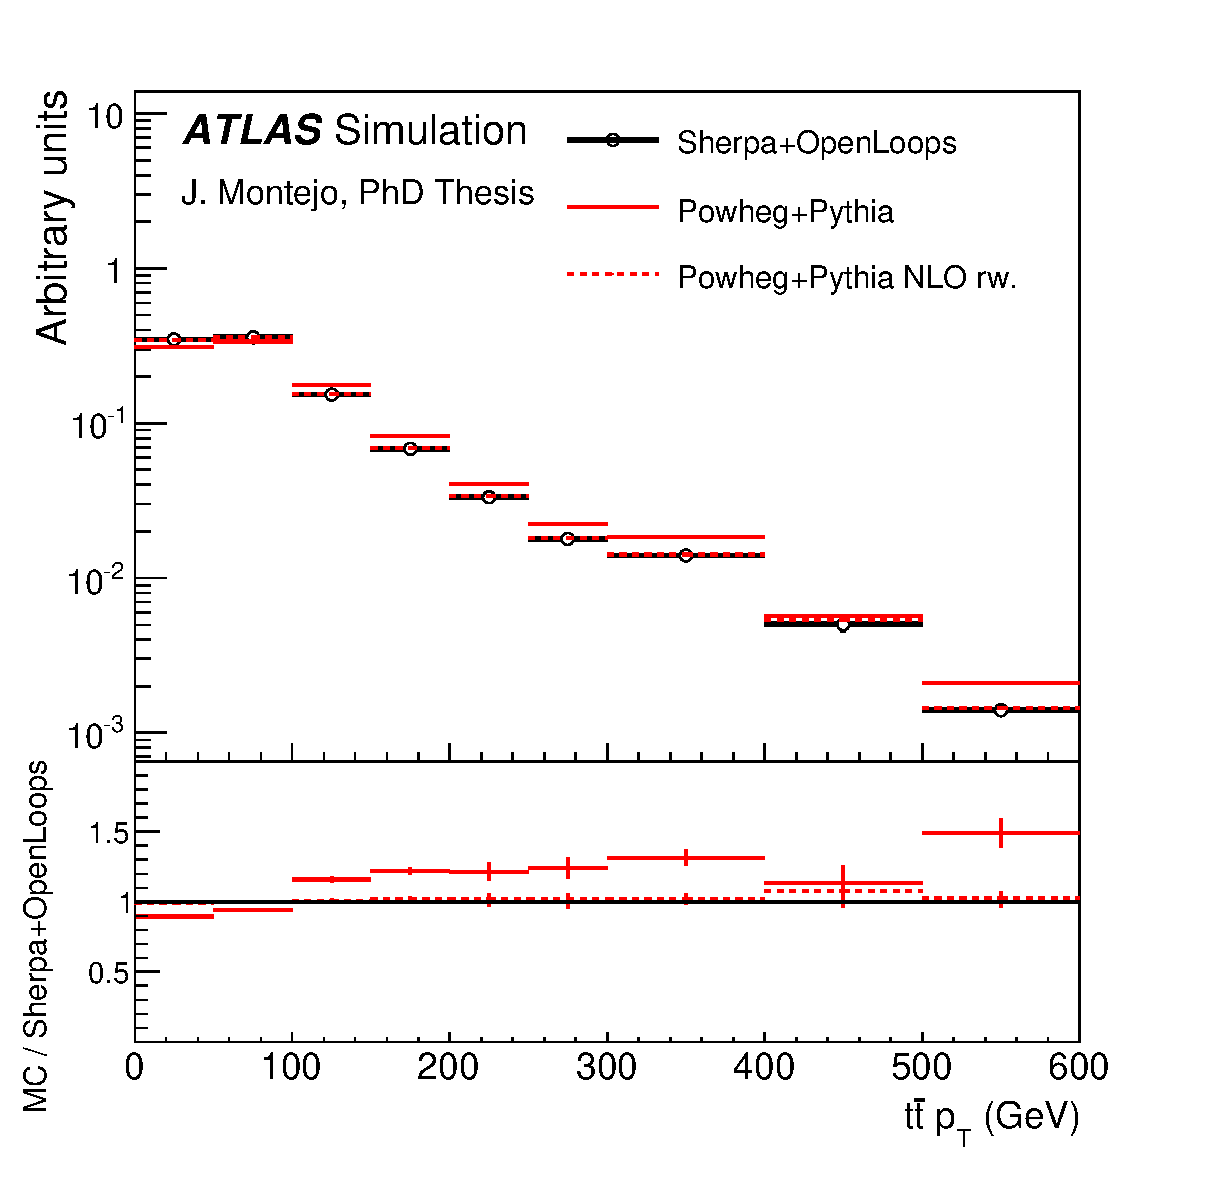
\includegraphics[width=0.48\textwidth]{Modeling/Figures/rw_tt1bq_ttbar_pt.eps} \\
\end{tabular}
\caption{Comparison of kinematic variables in the $t\bar{t}+b$ topology between \ShOL\ and \PP\ before (solid) and after (dashed) reweighting.}
\label{fig:default_tt1b_rw}
\end{center}
\end{figure}
\begin{figure}[p]
\begin{center}
\begin{tabular}{cc}
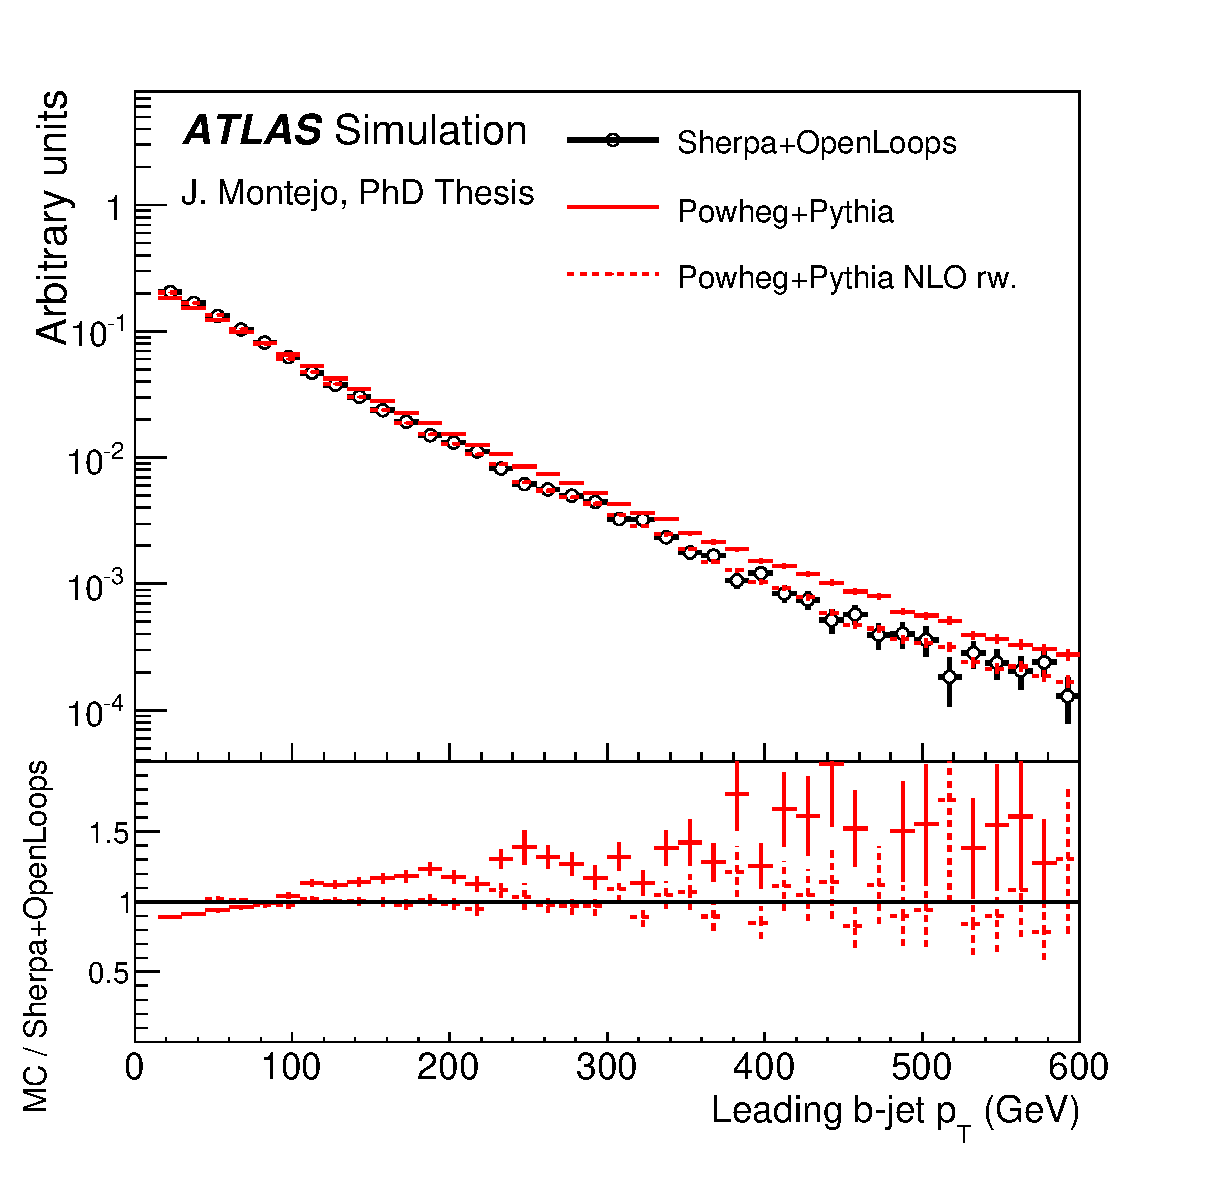
\includegraphics[width=0.48\textwidth]{Modeling/Figures/rw_tt1gbbq_q1_pt.eps} &
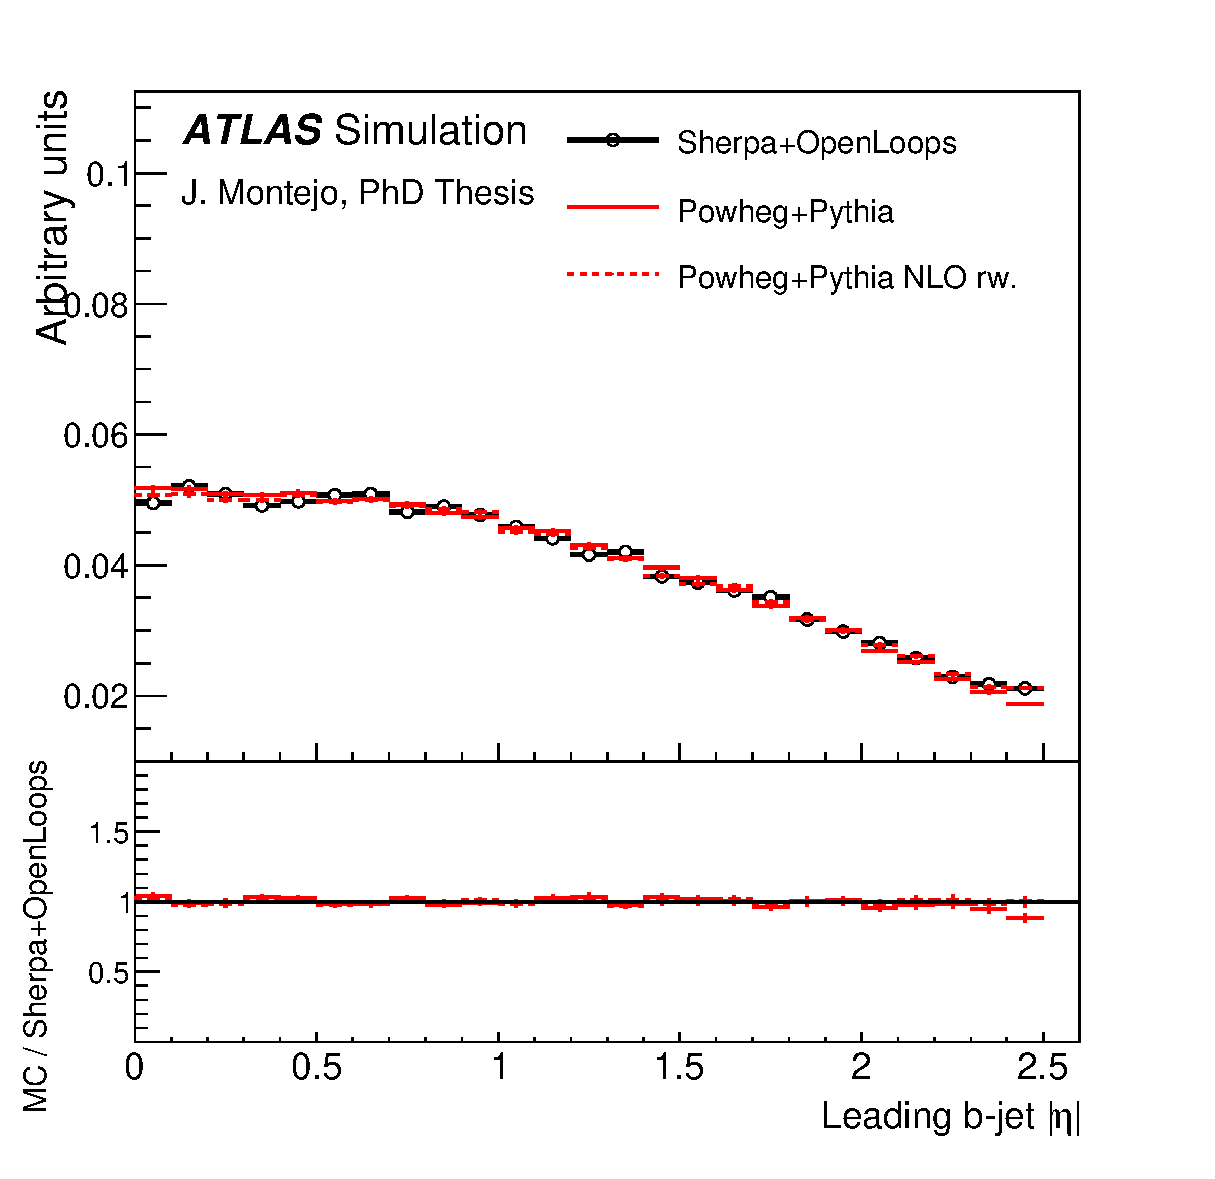
\includegraphics[width=0.48\textwidth]{Modeling/Figures/rw_tt1gbbq_q1_eta.eps} \\
\includegraphics[width=0.48\textwidth]{Modeling/Figures/rw_tt1gbbq_top_pt.eps} &
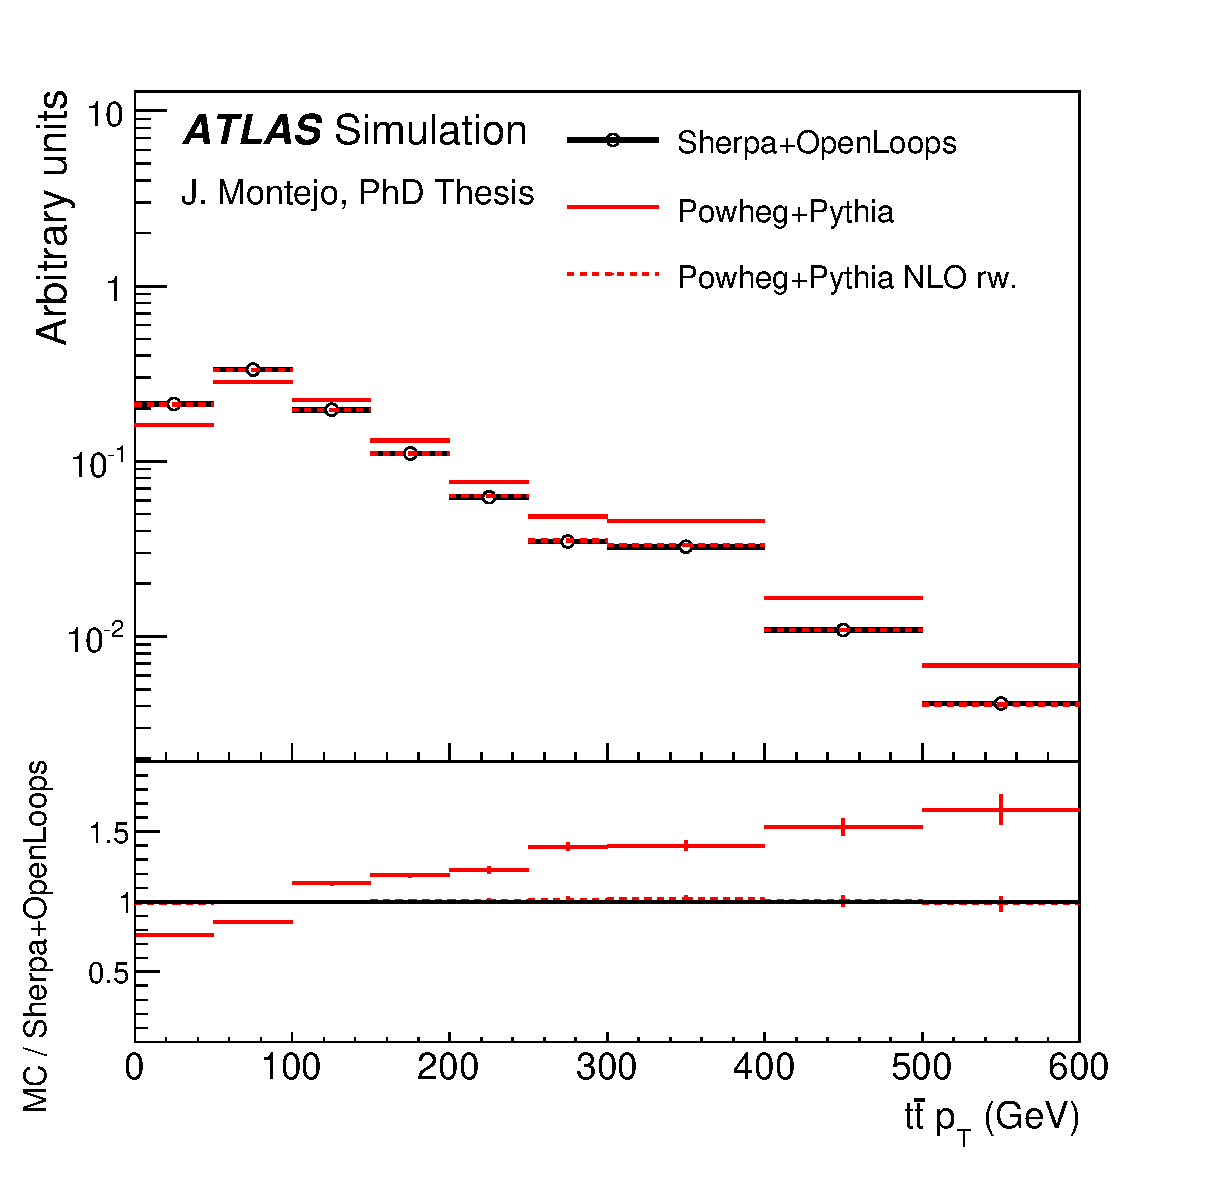
\includegraphics[width=0.48\textwidth]{Modeling/Figures/rw_tt1gbbq_ttbar_pt.eps} \\
\end{tabular}
\caption{Comparison of kinematic variables in the $t\bar{t}+B$ topology between \ShOL\ and \PP\ before (solid) and after (dashed) reweighting.}
\label{fig:default_tt1gbb_rw}
\end{center}
\end{figure}
\begin{figure}[p]
\begin{center}
\begin{tabular}{cc}
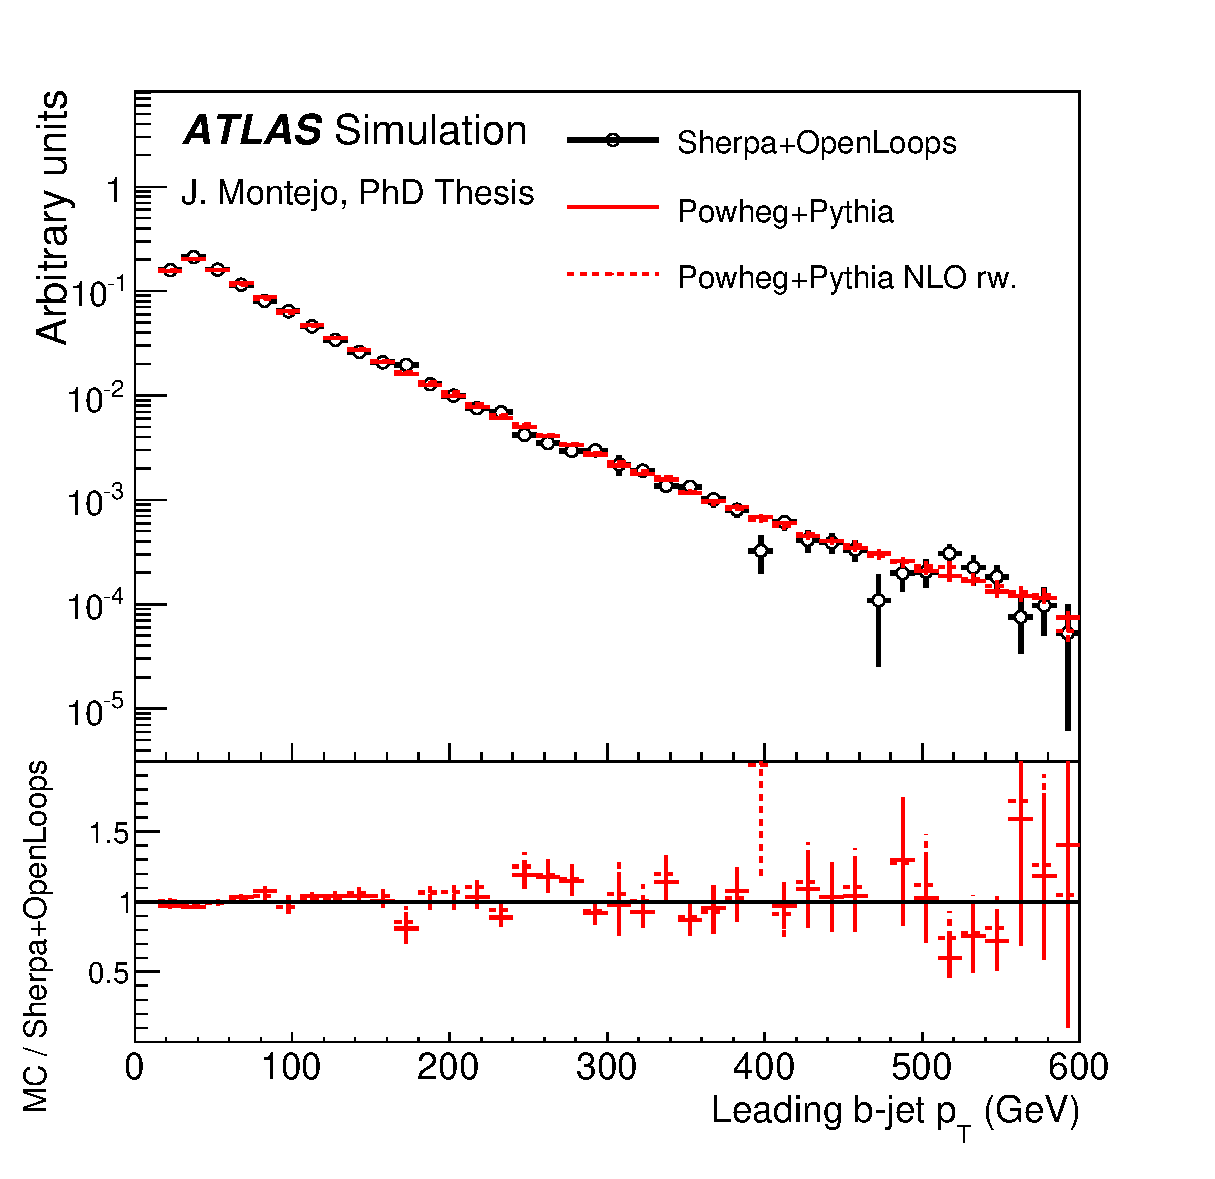
\includegraphics[width=0.48\textwidth]{Modeling/Figures/rw_ttbb_q1_pt.eps} &
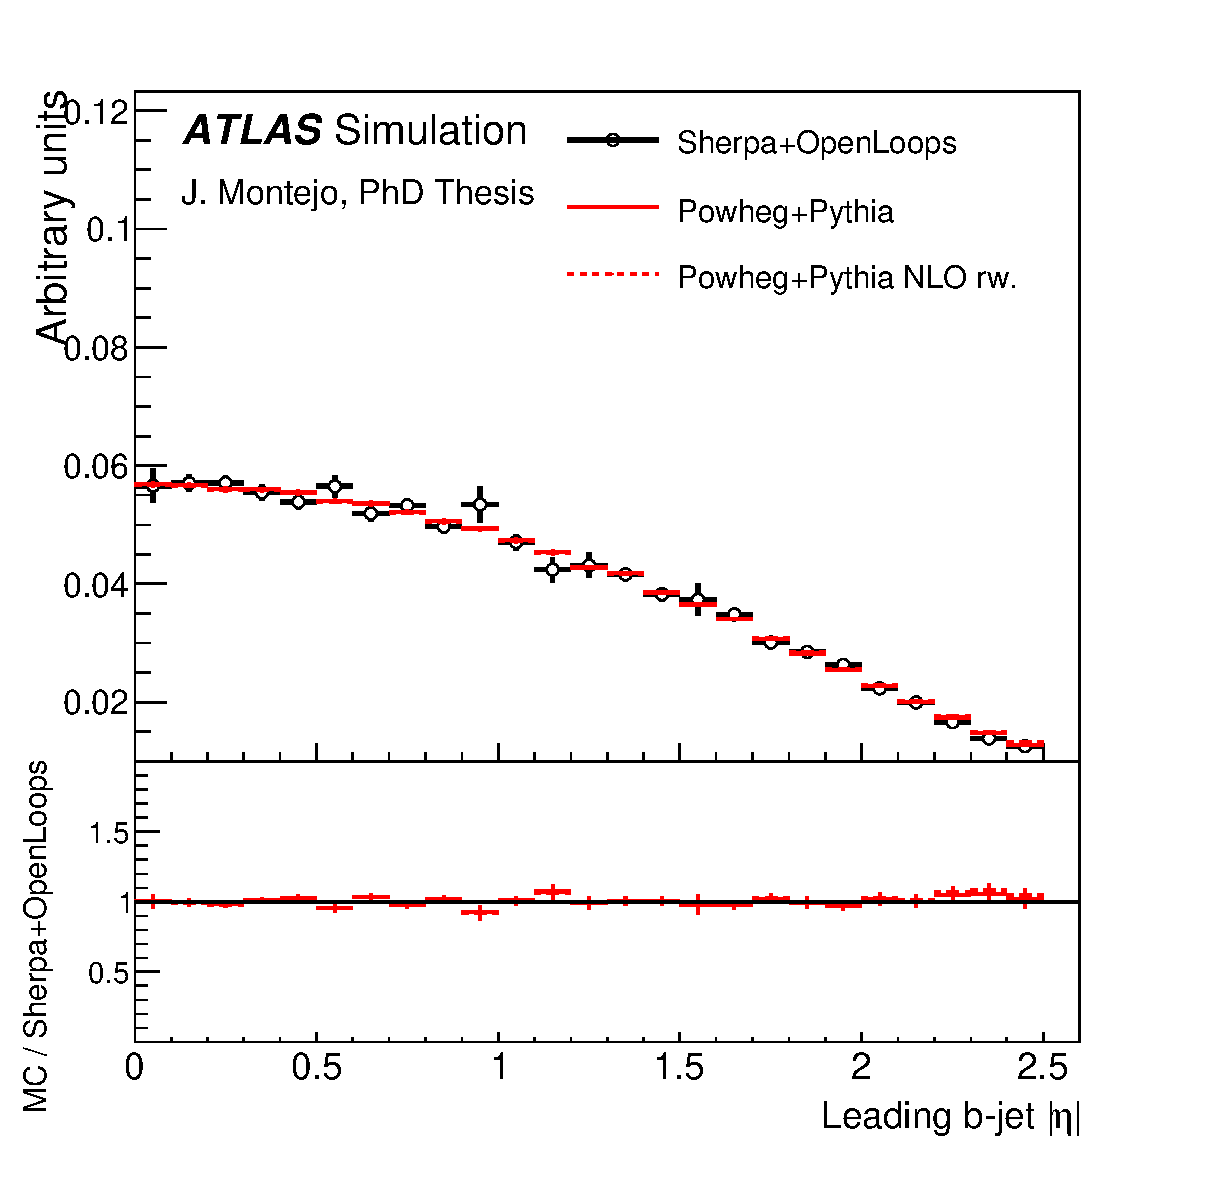
\includegraphics[width=0.48\textwidth]{Modeling/Figures/rw_ttbb_q1_eta.eps} \\
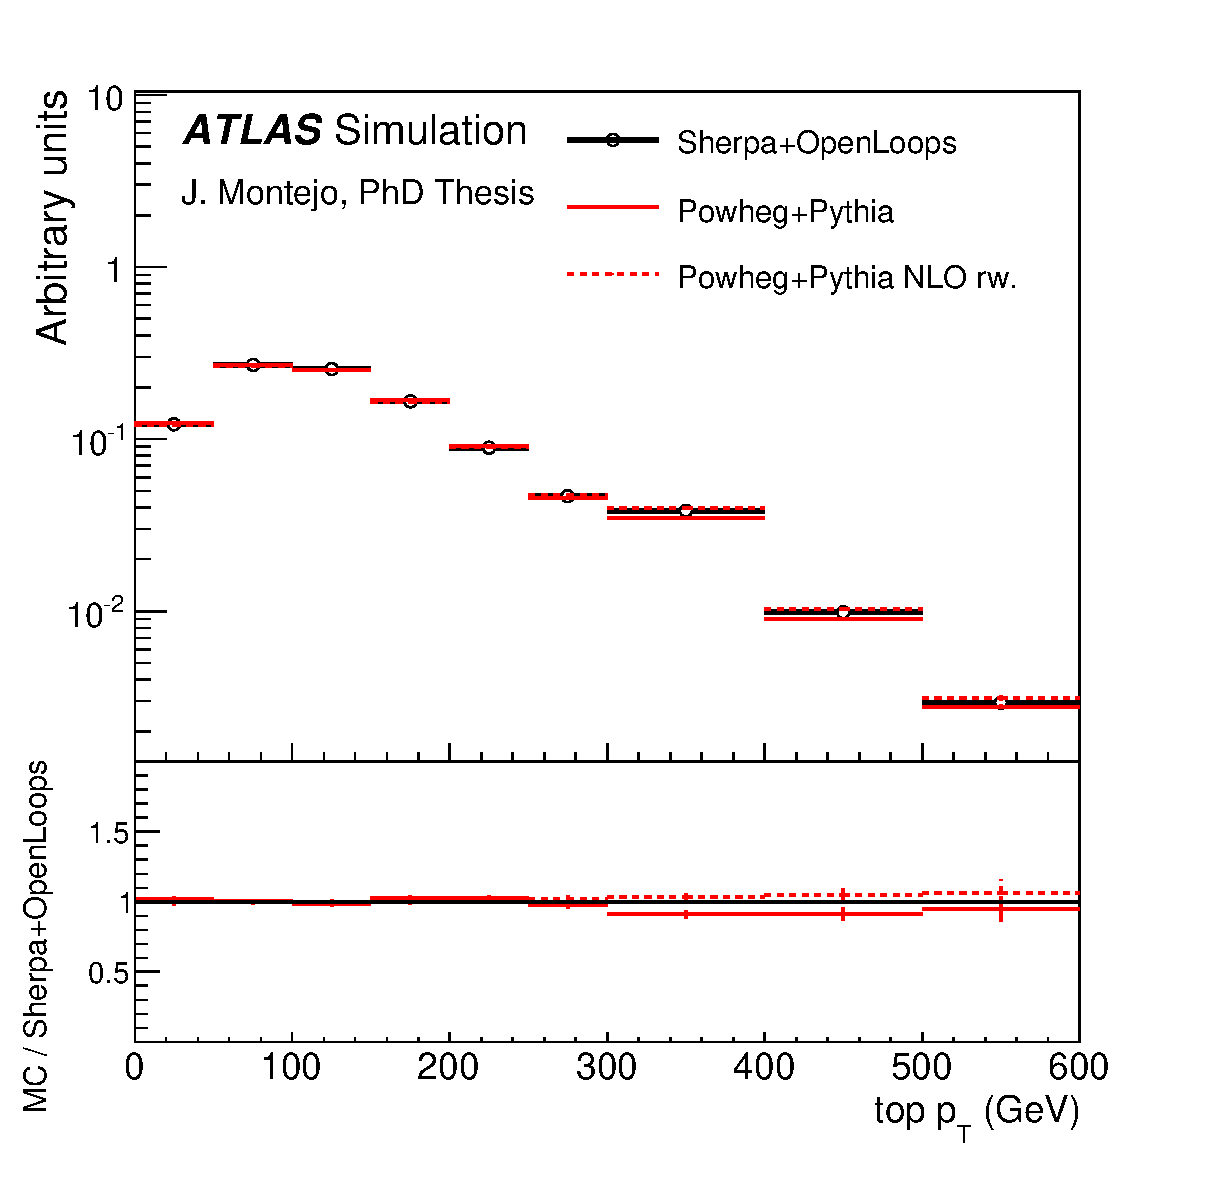
\includegraphics[width=0.48\textwidth]{Modeling/Figures/rw_ttbb_top_pt.eps} &
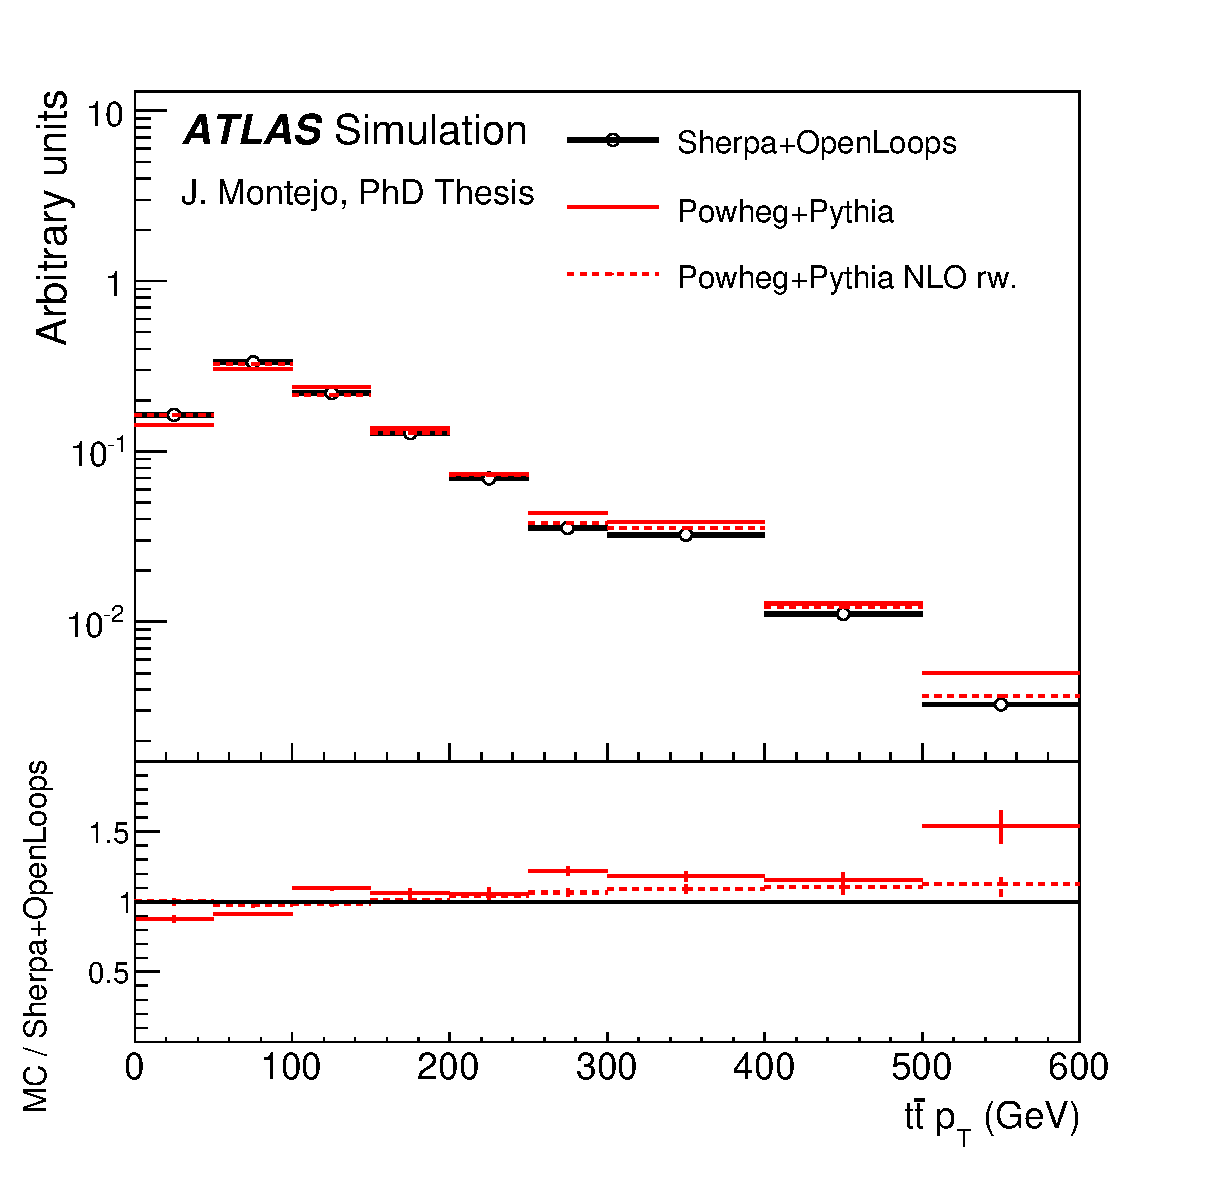
\includegraphics[width=0.48\textwidth]{Modeling/Figures/rw_ttbb_ttbar_pt.eps} \\
\end{tabular}
\caption{Comparison of kinematic variables in the $t\bar{t}+bb$ topology between \ShOL\ and \PP\ before (solid) and after (dashed) reweighting.}
\label{fig:default_tt2b_rw}
\end{center}
\end{figure}
\begin{figure}[p]
\begin{center}
\begin{tabular}{cc}
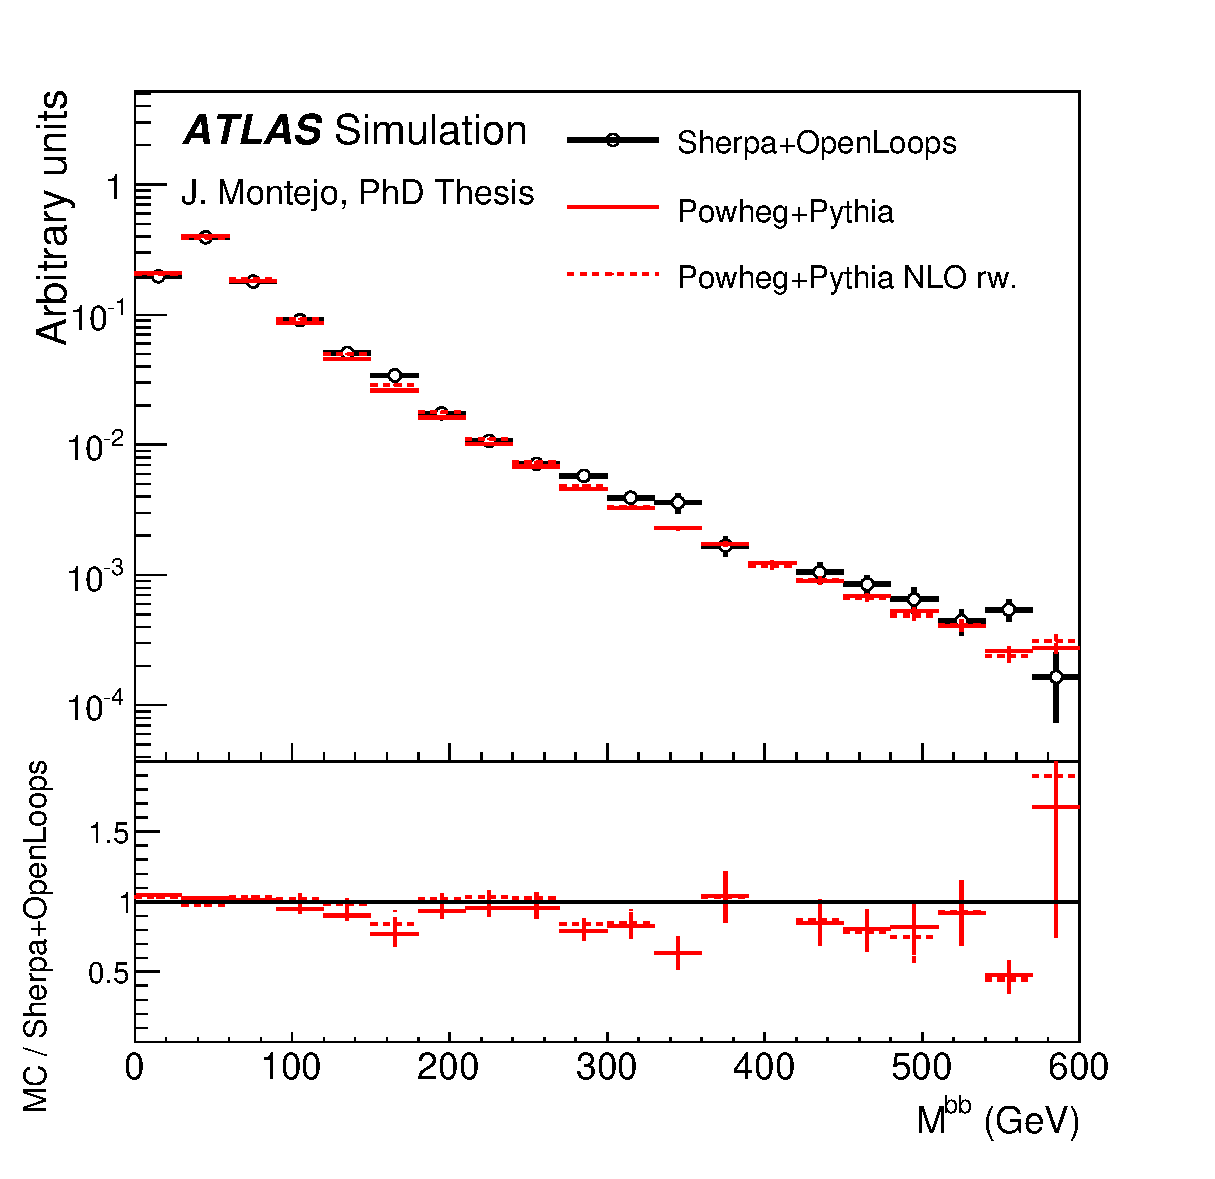
\includegraphics[width=0.48\textwidth]{Modeling/Figures/rw_ttbb_qq_m.eps} &
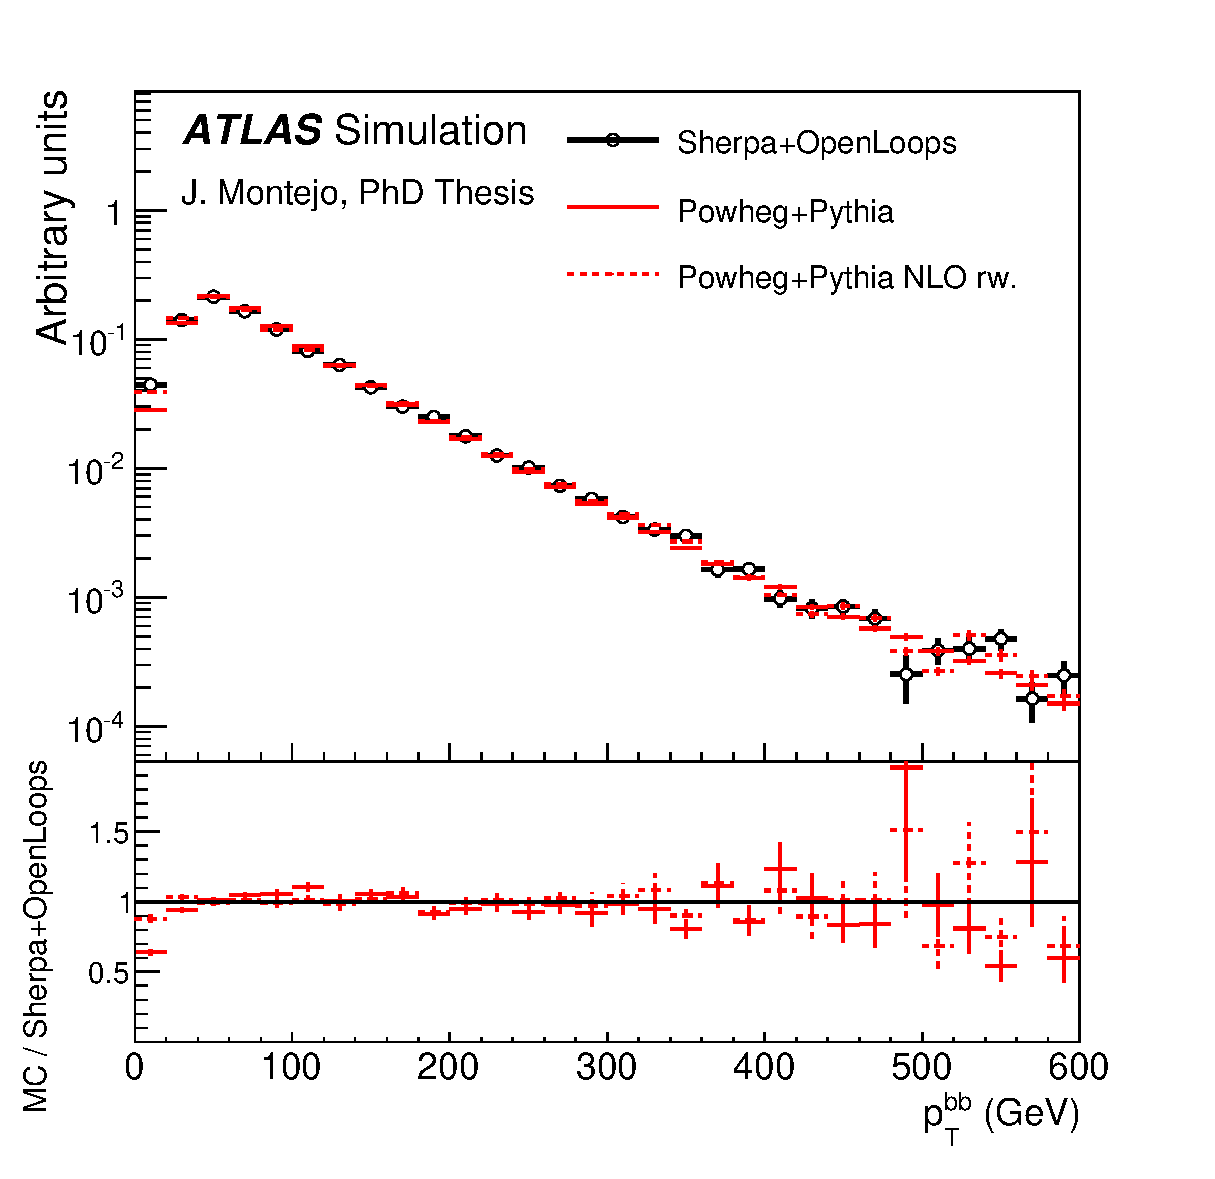
\includegraphics[width=0.48\textwidth]{Modeling/Figures/rw_ttbb_qq_pt.eps} \\
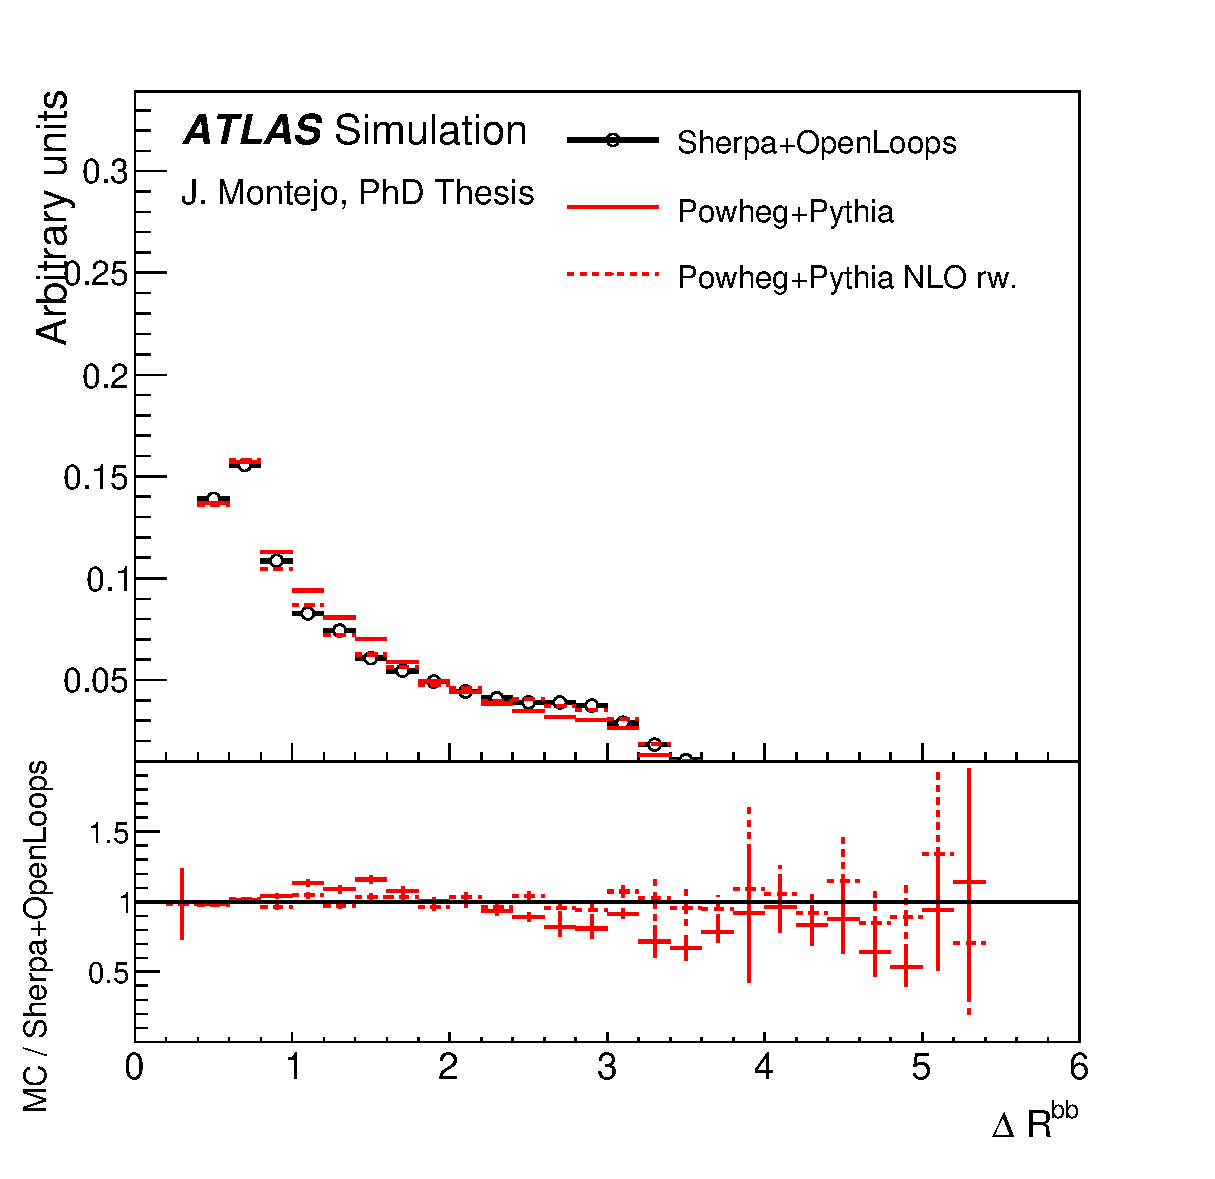
\includegraphics[width=0.48\textwidth]{Modeling/Figures/rw_ttbb_qq_dr.eps} &
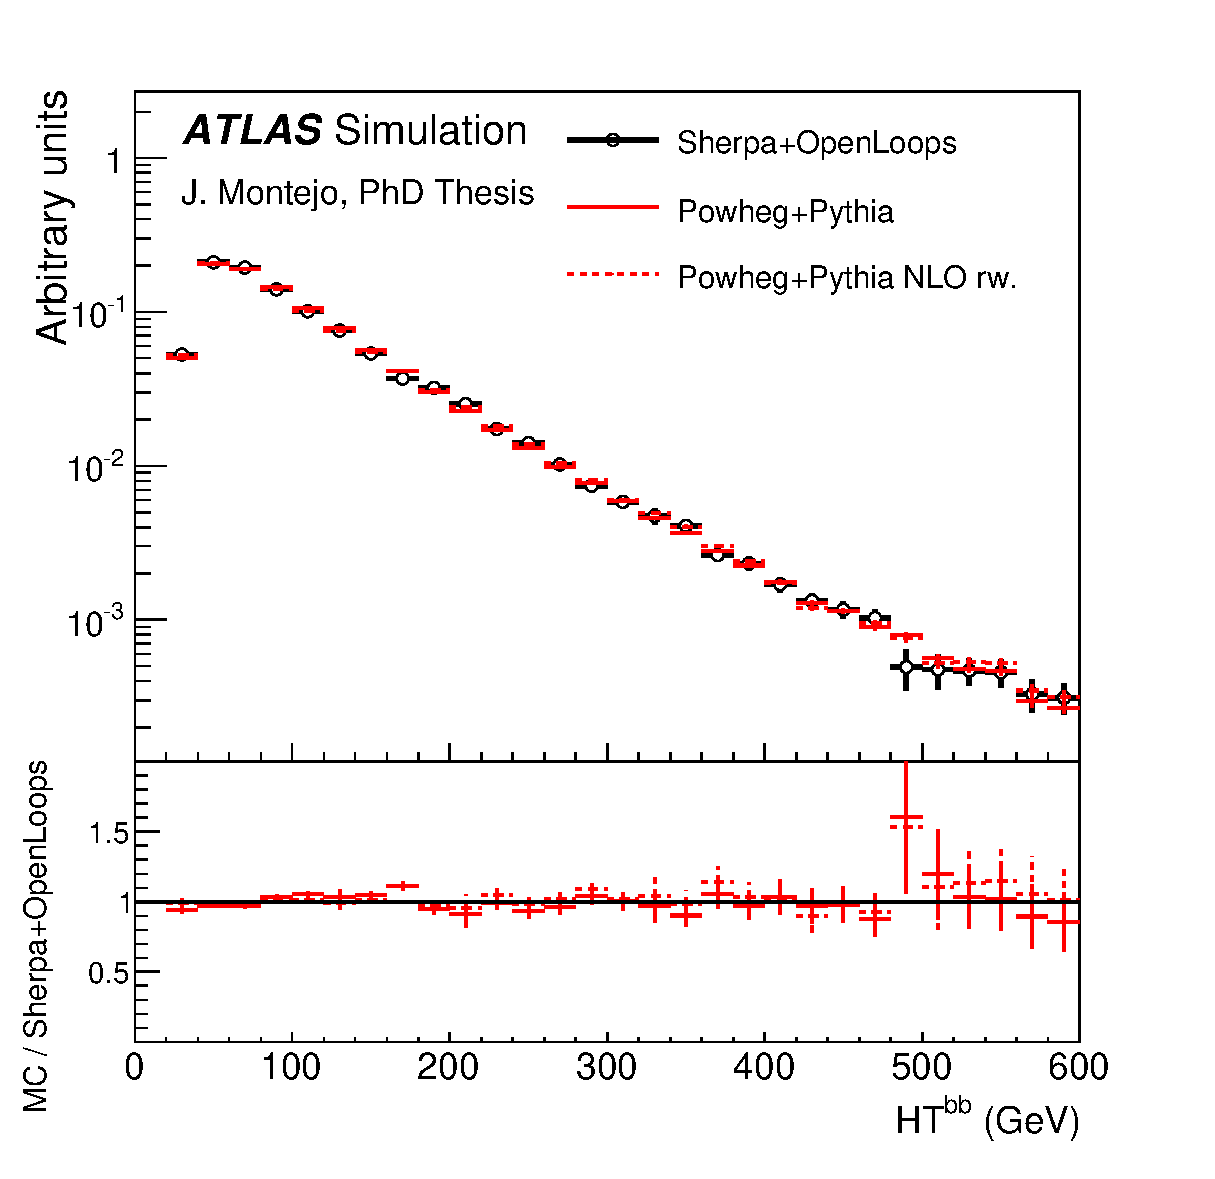
\includegraphics[width=0.48\textwidth]{Modeling/Figures/rw_ttbb_qq_ht.eps} \\
\end{tabular}
\caption{Comparison of kinematic variables of the \bbbar\ system in the $t\bar{t}+bb$ topology between \ShOL\ and \PP\ before (solid) and after (dashed) reweighting.}
\label{fig:default_tt2b_bb_rw}
\end{center}
\end{figure}
%%%%%%%%%%%%%% ttbb systematic
\begin{figure}[p]
\begin{center}
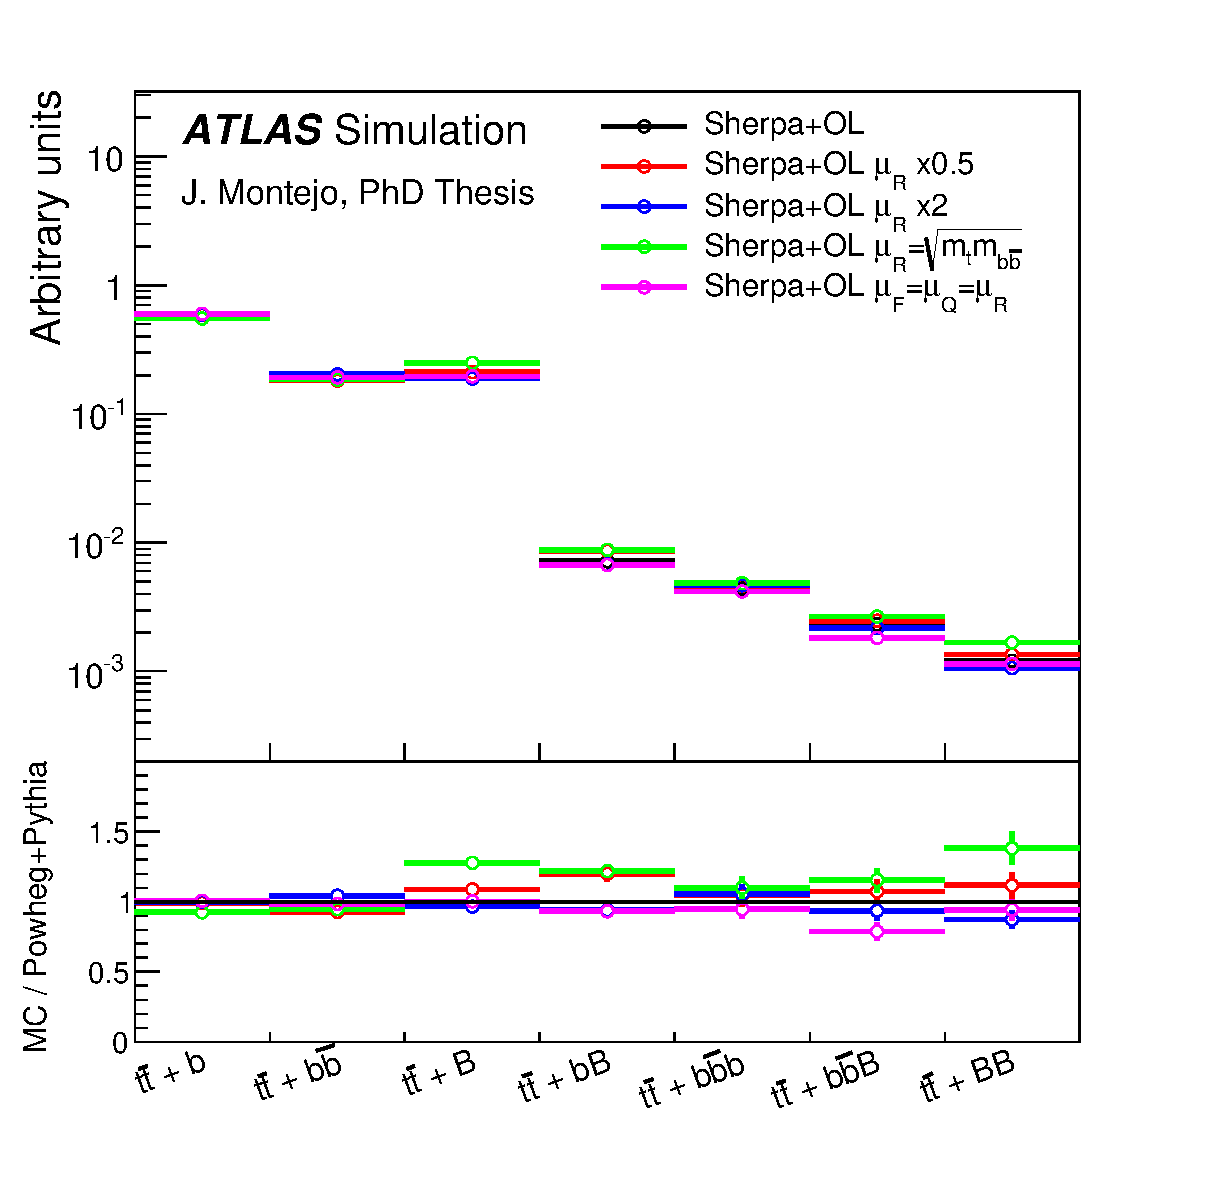
\includegraphics[width=0.6\textwidth]{Modeling/Figures/scales_realHFbb_extHFtype_norm.eps} \\
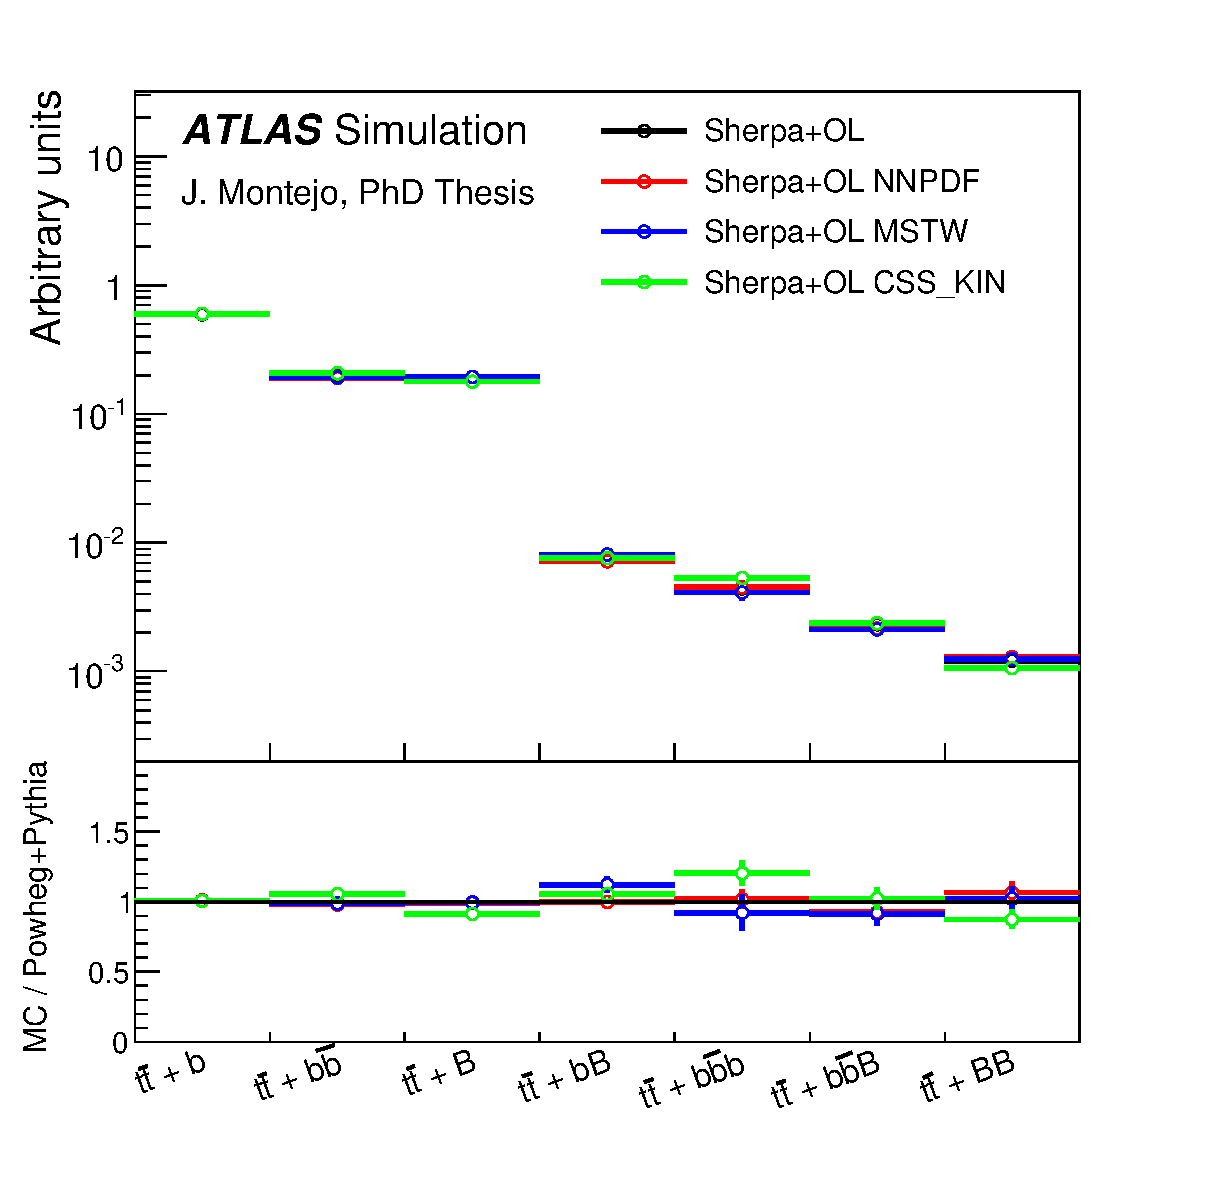
\includegraphics[width=0.6\textwidth]{Modeling/Figures/other_realHFbb_extHFtype_norm.eps} 
\caption{Effect of the scale variations, PDF variations and shower recoil scheme on \ShOL\ on the relative contribution of \ttbb\ subcategories.}
\label{fig:scales_other_extHFtype_app}
\end{center}
\end{figure}
\begin{figure}[p]
\begin{center}
\begin{tabular}{cc}
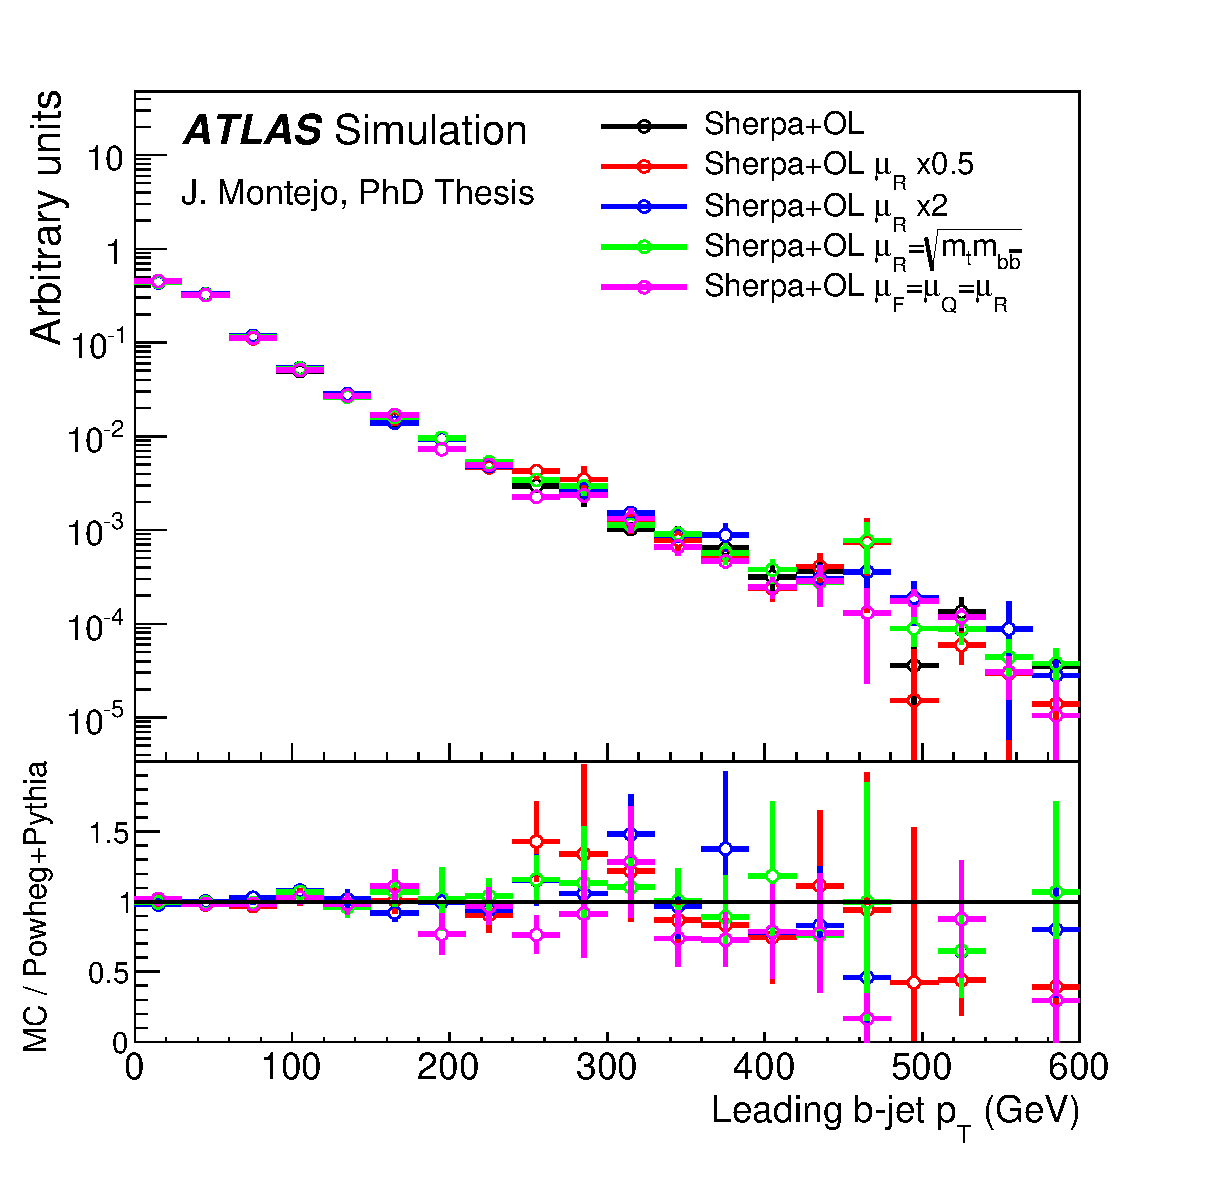
\includegraphics[width=0.48\textwidth]{Modeling/Figures/scales_tt1bq_q1_pt_norm} &
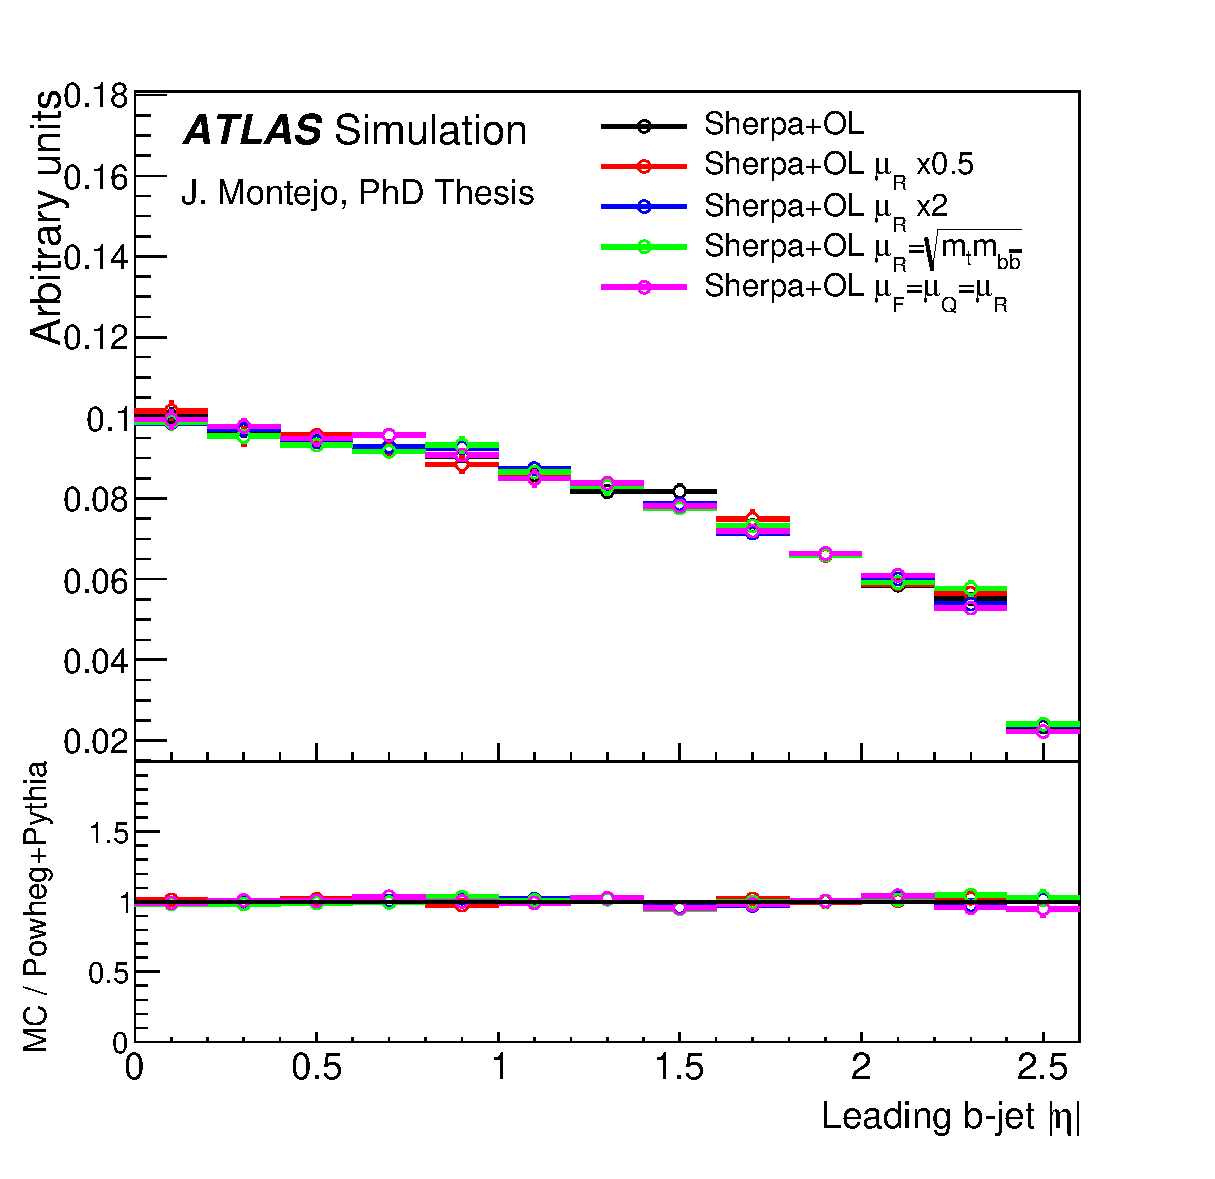
\includegraphics[width=0.48\textwidth]{Modeling/Figures/scales_tt1bq_q1_eta_norm} \\
\includegraphics[width=0.48\textwidth]{Modeling/Figures/scales_tt1bq_top_pt_norm} &
\includegraphics[width=0.48\textwidth]{Modeling/Figures/scales_tt1bq_ttbar_pt_norm} \\
\end{tabular}
\caption{Effect of the scale variations on \ShOL\ on kinematic variables in the $t\bar{t}+b$ topology.}
\label{fig:scales_tt1b}
\end{center}
\end{figure}
\begin{figure}[p]
\begin{center}
\begin{tabular}{cc}
\includegraphics[width=0.48\textwidth]{Modeling/Figures/other_tt1bq_q1_pt_norm} &
\includegraphics[width=0.48\textwidth]{Modeling/Figures/other_tt1bq_q1_eta_norm} \\
\includegraphics[width=0.48\textwidth]{Modeling/Figures/other_tt1bq_top_pt_norm} &
\includegraphics[width=0.48\textwidth]{Modeling/Figures/other_tt1bq_ttbar_pt_norm} \\
\end{tabular}
\caption{Effect of PDF variations and shower recoil scheme  on \ShOL\ on kinematic variables in the $t\bar{t}+b$ topology.}
\label{fig:other_tt1b}
\end{center}
\end{figure}
\begin{figure}[p]
\begin{center}
\begin{tabular}{cc}
\includegraphics[width=0.48\textwidth]{Modeling/Figures/scales_tt1gbbq_q1_pt_norm} &
\includegraphics[width=0.48\textwidth]{Modeling/Figures/scales_tt1gbbq_q1_eta_norm} \\
\includegraphics[width=0.48\textwidth]{Modeling/Figures/scales_tt1gbbq_top_pt_norm} &
\includegraphics[width=0.48\textwidth]{Modeling/Figures/scales_tt1gbbq_ttbar_pt_norm} \\
\end{tabular}
\caption{Effect of the scale variations  on \ShOL\ on kinematic variables in the $t\bar{t}+B$ topology.}
\label{fig:scales_tt1gbb}
\end{center}
\end{figure}
\begin{figure}[p]
\begin{center}
\begin{tabular}{cc}
\includegraphics[width=0.48\textwidth]{Modeling/Figures/other_tt1gbbq_q1_pt_norm} &
\includegraphics[width=0.48\textwidth]{Modeling/Figures/other_tt1gbbq_q1_eta_norm} \\
\includegraphics[width=0.48\textwidth]{Modeling/Figures/other_tt1gbbq_top_pt_norm} &
\includegraphics[width=0.48\textwidth]{Modeling/Figures/other_tt1gbbq_ttbar_pt_norm} \\
\end{tabular}
\caption{Effect of PDF variations and shower recoil scheme  on \ShOL\ on kinematic variables in the $t\bar{t}+B$ topology.}
\label{fig:other_tt1gbb}
\end{center}
\end{figure}
\begin{figure}[p]
\begin{center}
\begin{tabular}{cc}
\includegraphics[width=0.48\textwidth]{Modeling/Figures/scales_tt2bq_q1_pt_norm} &
\includegraphics[width=0.48\textwidth]{Modeling/Figures/scales_tt2bq_q1_eta_norm} \\
\includegraphics[width=0.48\textwidth]{Modeling/Figures/scales_tt2bq_top_pt_norm} &
\includegraphics[width=0.48\textwidth]{Modeling/Figures/scales_tt2bq_ttbar_pt_norm} \\
\end{tabular}
\caption{Effect of the scale variations  on \ShOL\ on kinematic variables in the \ttbb\ topology.}
\label{fig:scales_tt2b}
\end{center}
\end{figure}
\begin{figure}[p]
\begin{center}
\begin{tabular}{cc}
\includegraphics[width=0.48\textwidth]{Modeling/Figures/other_tt2bq_q1_pt_norm} &
\includegraphics[width=0.48\textwidth]{Modeling/Figures/other_tt2bq_q1_eta_norm} \\
\includegraphics[width=0.48\textwidth]{Modeling/Figures/other_tt2bq_top_pt_norm} &
\includegraphics[width=0.48\textwidth]{Modeling/Figures/other_tt2bq_ttbar_pt_norm} \\
\end{tabular}
\caption{Effect of PDF variations and shower recoil scheme  on \ShOL\ on kinematic variables in the \ttbb\ topology.}
\label{fig:other_tt2b}
\end{center}
\end{figure}
\begin{figure}[p]
\begin{center}
\begin{tabular}{cc}
\includegraphics[width=0.48\textwidth]{Modeling/Figures/scales_tt2bq_qq_m_norm} &
\includegraphics[width=0.48\textwidth]{Modeling/Figures/scales_tt2bq_qq_pt_norm} \\
\includegraphics[width=0.48\textwidth]{Modeling/Figures/scales_tt2bq_qq_dr_norm} &
\includegraphics[width=0.48\textwidth]{Modeling/Figures/scales_tt2bq_qq_ht_norm} \\
\end{tabular}
\caption{Effect of the scale variations  on \ShOL\ on kinematic variables of the \bbbar\ system in the \ttbb\ topology.}
\label{fig:scales_tt2b_bb}
\end{center}
\end{figure}
\begin{figure}[p]
\begin{center}
\begin{tabular}{cc}
\includegraphics[width=0.48\textwidth]{Modeling/Figures/other_tt2bq_qq_m_norm} &
\includegraphics[width=0.48\textwidth]{Modeling/Figures/other_tt2bq_qq_pt_norm} \\
\includegraphics[width=0.48\textwidth]{Modeling/Figures/other_tt2bq_qq_dr_norm} &
\includegraphics[width=0.48\textwidth]{Modeling/Figures/other_tt2bq_qq_ht_norm} \\
\end{tabular}
\caption{Effect of PDF variations and shower recoil scheme  on \ShOL\ on kinematic variables of the \bbbar\ system in the \ttbb\ topology.}
\label{fig:other_tt2b_bb}
\end{center}
\end{figure}

%%%%%%%%%%%%%%% ttcc basic
\begin{figure}[p]
\begin{center}
\includegraphics[width=0.46\textwidth]{Modeling/Figures/defaultcc_realHFcc_extHFtype_ttcc_norm.eps}
\caption{Comparison of \ttcc\ subcategories between \PP\ and \madgraph+\pythia.}
\label{fig:defaultcc_extHFtype_app}
\end{center}
\vspace{-20pt}
\begin{center}
\begin{tabular}{cc}
\includegraphics[width=0.46\textwidth]{Modeling/Figures/defaultcc_tt1cq_q1_pt_norm.eps} &
\includegraphics[width=0.46\textwidth]{Modeling/Figures/defaultcc_tt1cq_q1_eta_norm.eps} \\
\includegraphics[width=0.46\textwidth]{Modeling/Figures/defaultcc_tt1cq_top_pt_norm.eps} &
\includegraphics[width=0.46\textwidth]{Modeling/Figures/defaultcc_tt1cq_ttbar_pt_norm.eps} \\
\end{tabular}
\caption{Comparison of kinematic variables in the $t\bar{t}+c$ topology between \PP\ and \madgraph+\pythia.}
\label{fig:defaultcc_tt1c}
\end{center}
\end{figure}
\begin{figure}[p]
\begin{center}
\begin{tabular}{cc}
\includegraphics[width=0.48\textwidth]{Modeling/Figures/defaultcc_tt1gccq_q1_pt_norm.eps} &
\includegraphics[width=0.48\textwidth]{Modeling/Figures/defaultcc_tt1gccq_q1_eta_norm.eps} \\
\includegraphics[width=0.48\textwidth]{Modeling/Figures/defaultcc_tt1gccq_top_pt_norm.eps} &
\includegraphics[width=0.48\textwidth]{Modeling/Figures/defaultcc_tt1gccq_ttbar_pt_norm.eps} \\
\end{tabular}
\caption{Comparison of kinematic variables in the $t\bar{t}+C$ topology between \PP\ and \madgraph+\pythia.}
\label{fig:defaultcc_tt1gcc}
\end{center}
\end{figure}
\begin{figure}[p]
\begin{center}
\begin{tabular}{cc}
\includegraphics[width=0.48\textwidth]{Modeling/Figures/defaultcc_tt2cq_q1_pt_norm.eps} &
\includegraphics[width=0.48\textwidth]{Modeling/Figures/defaultcc_tt2cq_q1_eta_norm.eps} \\
\includegraphics[width=0.48\textwidth]{Modeling/Figures/defaultcc_tt2cq_top_pt_norm.eps} &
\includegraphics[width=0.48\textwidth]{Modeling/Figures/defaultcc_tt2cq_ttbar_pt_norm.eps} \\
\end{tabular}
\caption{Comparison of kinematic variables in the $t\bar{t}+cc$ topology between \PP\ and \madgraph+\pythia.}
\label{fig:defaultcc_tt2c}
\end{center}
\end{figure}
\begin{figure}[p]
\begin{center}
\begin{tabular}{cc}
\includegraphics[width=0.48\textwidth]{Modeling/Figures/defaultcc_tt2cq_qq_m_norm.eps} &
\includegraphics[width=0.48\textwidth]{Modeling/Figures/defaultcc_tt2cq_qq_pt_norm.eps} \\
\includegraphics[width=0.48\textwidth]{Modeling/Figures/defaultcc_tt2cq_qq_dr_norm.eps} &
\includegraphics[width=0.48\textwidth]{Modeling/Figures/defaultcc_tt2cq_qq_ht_norm.eps} \\
\end{tabular}
\caption{Comparison of kinematic variables of the \ccbar\ system in the $t\bar{t}+cc$ topology between \PP\ and \madgraph+\pythia.}
\label{fig:defaultcc_tt2c_cc}
\end{center}
\end{figure}
%%%%%%%%%%%%%% ttcc systematic
\begin{figure}[p]
\begin{center}
\includegraphics[width=0.46\textwidth]{Modeling/Figures/mgcc_realHFcc_extHFtype_ttcc_norm.eps}
\caption{Effect of the systematic variations on \madgraph+\pythia\ on the \ttcc\ subcategories.}
\label{fig:mgcc_extHFtype_app}
\end{center}
\vspace{-20pt}
\begin{center}
\begin{tabular}{cc}
\includegraphics[width=0.46\textwidth]{Modeling/Figures/mgcc_tt1cq_q1_pt_norm.eps} &
\includegraphics[width=0.46\textwidth]{Modeling/Figures/mgcc_tt1cq_q1_eta_norm.eps} \\
\includegraphics[width=0.46\textwidth]{Modeling/Figures/mgcc_tt1cq_top_pt_norm.eps} &
\includegraphics[width=0.46\textwidth]{Modeling/Figures/mgcc_tt1cq_ttbar_pt_norm.eps} \\
\end{tabular}
\caption{Effect of the systematic variations on \madgraph+\pythia\ on kinematic variables in the \ttc\ topology.}
\label{fig:mgcc_tt1c}
\end{center}
\end{figure}
\begin{figure}[p]
\begin{center}
\begin{tabular}{cc}
\includegraphics[width=0.48\textwidth]{Modeling/Figures/mgcc_tt1gccq_q1_pt_norm.eps} &
\includegraphics[width=0.48\textwidth]{Modeling/Figures/mgcc_tt1gccq_q1_eta_norm.eps} \\
\includegraphics[width=0.48\textwidth]{Modeling/Figures/mgcc_tt1gccq_top_pt_norm.eps} &
\includegraphics[width=0.48\textwidth]{Modeling/Figures/mgcc_tt1gccq_ttbar_pt_norm.eps} \\
\end{tabular}
\caption{Effect of the systematic variations on \madgraph+\pythia\ on kinematic variables in the \ttC\ topology.}
\label{fig:mgcc_tt1gcc}
\end{center}
\end{figure}
\begin{figure}[p]
\begin{center}
\begin{tabular}{cc}
\includegraphics[width=0.48\textwidth]{Modeling/Figures/mgcc_tt2cq_q1_pt_norm.eps} &
\includegraphics[width=0.48\textwidth]{Modeling/Figures/mgcc_tt2cq_q1_eta_norm.eps} \\
\includegraphics[width=0.48\textwidth]{Modeling/Figures/mgcc_tt2cq_top_pt_norm.eps} &
\includegraphics[width=0.48\textwidth]{Modeling/Figures/mgcc_tt2cq_ttbar_pt_norm.eps} \\
\end{tabular}
\caption{Effect of the systematic variations on \madgraph+\pythia\ on kinematic variables in the \ttcc\ topology.}
\label{fig:mgcc_tt2c}
\end{center}
\end{figure}
\begin{figure}[p]
\begin{center}
\begin{tabular}{cc}
\includegraphics[width=0.48\textwidth]{Modeling/Figures/mgcc_tt2cq_qq_m_norm.eps} &
\includegraphics[width=0.48\textwidth]{Modeling/Figures/mgcc_tt2cq_qq_pt_norm.eps} \\
\includegraphics[width=0.48\textwidth]{Modeling/Figures/mgcc_tt2cq_qq_dr_norm.eps} &
\includegraphics[width=0.48\textwidth]{Modeling/Figures/mgcc_tt2cq_qq_ht_norm.eps} \\
\end{tabular}
\caption{Effect of the systematic variations on \madgraph+\pythia\ on kinematic variables of the \ccbar\ system in the \ttcc\ topology.}
\label{fig:mgcc_tt2c_cc}
\end{center}
\end{figure}
